

\chapter{METODOLOGI}
\label{sec:chap3_metodologi}



\section*{ }
Pada penelitian yang berjudul "Segmentasi Gumpalan Darah Vena Pada Citra \textit{Ultrasound} Menggunakan U-Net" nantinya akan terdiri dari empat langkah utama yaitu (1) data 2D citra \textit{ultrasound} gumpalan darah; (2) \textit{preprocessing}; (3) segmentasi gumpalan darah; serta (4) visualisasi 3D gumpala darah. Adapun empat langkah utama tersebut dapat dilihat pada Gambar \ref{fig:blokdiagram}.
\begin{figure}[H]
	\centering
	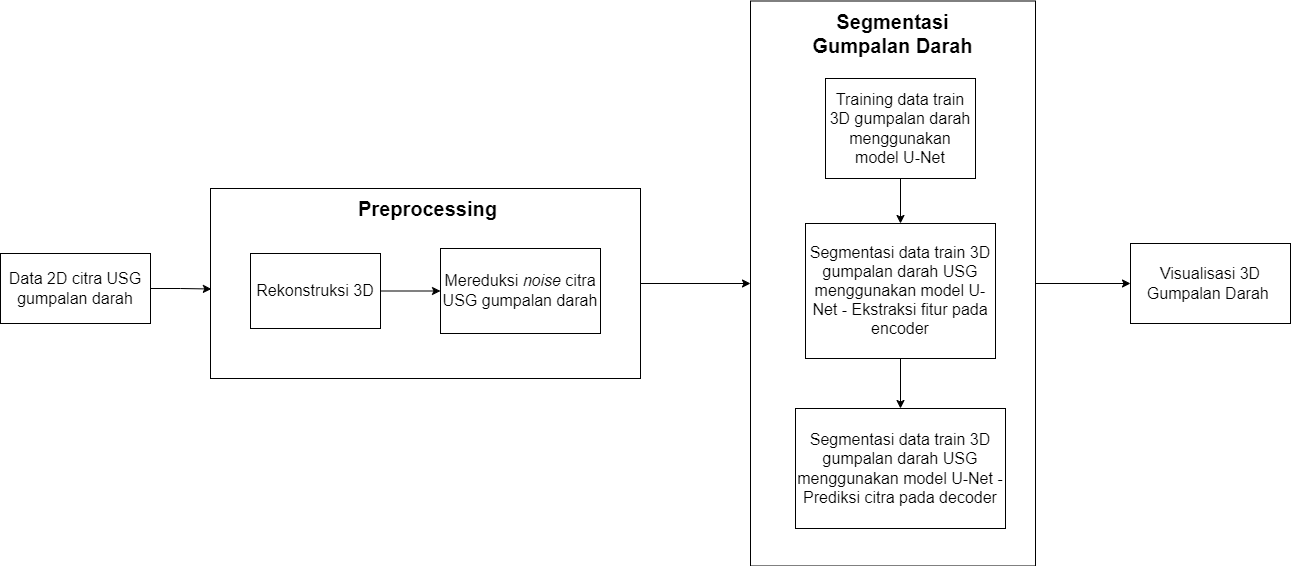
\includegraphics[width=\linewidth]{bab3/diagram-block version 2.png}
	\caption{Blok Diagram Segmentasi Gumpalan Darah Vena Pada Citra Ultrasound Menggunakan U-Net}
	\label{fig:blokdiagram}
\end{figure}


\section{Data 2D Citra \textit{Ultrasound} Gumpalan Darah Vena}

Data 2D citra ultrasound gumpalan darah (\textit{thrombus}) pada pembuluh darah vena diperoleh dari lima pasien dari penderita \textit{Deep Vein Thrombosis} (DVT) serta hasil akuisisi citra 2D ultrasound menggunakan peralatan seperti \textit{phantom}, USG \textit{Telemed-SmartUs}, \textit{Probe}, serta \textit{Optitrack}. Aturan dan syarat tertentu harus diikuti dalam penelitian ini sebelum memulai proses akuisisi citra ultrasound, untuk memastikan bahwa prosedur tersebut berjalan dengan baik. 

\subsection{Perangkat Akuisisi Citra \textit{Ultrasound} Gumpalan Darah Vena}
Penelitian ini menggunakan data citra ultrasound dua dimensi (2D) gumpalan darah (\textit{thrombus}) yang ada pada pembuluh darah vena. Data ini diakuisisi dari phantom yang terbuat dari balon panjang. Phantom balon panjang dirancang khusus oleh peneliti agar menyerupai bentuk pembuluh darah vena manusia, dan di dalamnya dimasukkan lemak sapi. Penggunaan lemak sapi dipilih karena struktur lemak sapi menyerupai bentuk \textit{thrombus} yang biasa ditemui di dalam pembuluh darah pasien penderita DVT. 

Penggunaan \textit{phantom} balon panjang ini bertujuan untuk menciptakan kondisi yang mirip dengan kondisi penderita DVT dimana \textit{thrombus} terbentuk di dalam pembuluh darah vena. Serta peneliti juga mengamati dan menganalisis bentuk \textit{thrombus} melalui citra ultrasound. Oleh karena itu penggunaan \textit{phantom} balon panjang sangat penting karena menjadi sumber utama  simulasi \textit{thrombus} yang terdapat pada pembuluh darah vena. Adapun \textit{phantom} balon panjang yang digunakan dalam penelitian ini serta hasil pencitraan \textit{ultrasound} menggunakan \textit{phantom} balon panjang dapat dilihat pada Gambar \ref{Fig:phantom_baloon}

\begin{figure}[h]
        \centering
	\begin{tabular}{ll}
		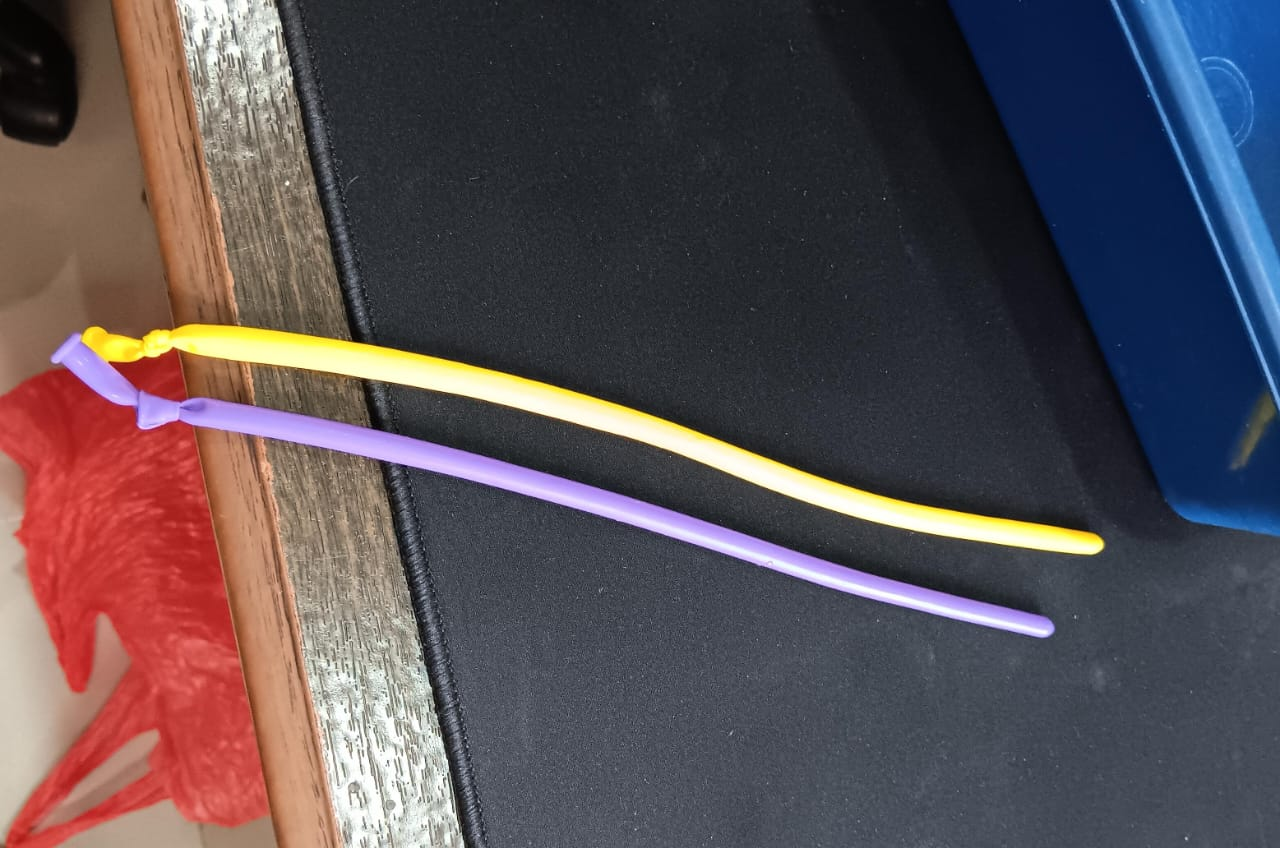
\includegraphics[scale=0.18]{bab3/phantom_balon.jpg}
		&
		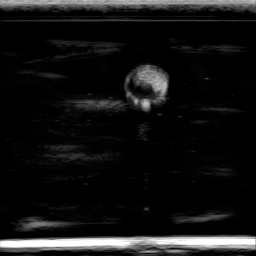
\includegraphics[scale=0.6]{bab3/img_thrombus.png} \\
		\multicolumn{1}{c}{(a)} & \multicolumn{1}{c}{(b)}
	\end{tabular}
	\caption{(a) \textit{Phantom} Balon Panjang (b) Hasil Pencitraan \textit{Ultrasound} Menggunakan \textit{Phantom} Balon Panjang.}
	\label{Fig:phantom_baloon}
\end{figure}

Selain menggunakan \textit{phantom} balon panjang, dalam beberapa percobaan peneliti menggunakan data \textit{thrombus} pada pembuluh darah vena yang diperoleh dari lima pasien penderita DVT dengan total 317 citra. \textit{Thrombus} penderita DVT terbentuk di dalam pembuluh darah vena bagian kaki. Data \textit{thrombus} ini menyajikan informasi visual yang dihasilkan dari pemindaian menggunakan sensor ultrasonografi (USG) yang memperlihatkan lokasi dan karakteristik \textit{thrombus} dalam pembuluh darah vena pada ke lima pasien tersebut.Penggunaan data penderita DVT ini bertujuan untuk meningkatkan variasi dalam dataset yang diterapkan selama pelatihan model \textit{deep learning} U-Net, sehingga model tersebut bisa melakukan segmentasi area gumpalan darah pada area pembuluh darah vena dengan tingkat keakuratan yang lebih tinggi. Adapun citra ultrasound \textit{thrombus} penderita DVT dapat dilihat pada Gambar \ref{fig:gumpalandarah}

\begin{figure}[H]
	\centering
	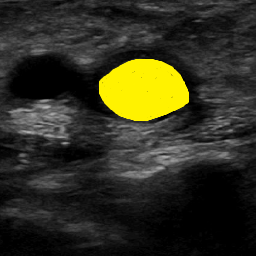
\includegraphics[scale= 0.7]{bab3/thrombus.png}
	\caption{Data Citra Ultrasound Gumpalan Darah}
	\label{fig:gumpalandarah}
\end{figure}

Data citra 2D \textit{ultrasound thrombus} menggunakan modalitas \textit{ultrasound} \textit{Telemed SmartUs EXT-1M} dan perangkat lunak \textit{Echowave II}. Fungsi dari modalitas \textit{ultrasound} \textit{Telemed SmartUs EXT-1M} adalah alat portable untuk mengakuisisi citra ultrasound guna melihat gambaran di dalam tubuh tanpa harus melakukan pembedahan. Echowave II merupakan perangkat lunak yang digunakan secara bersamaan dengan modalitas \textit{ultrasound} \textit{Telemed SmartUs EXT-1M} dan berfungsi untuk menangani pemrosesan data yang dikumpulkan oleh probe menjadi citra yang jelas dan dapat diinterpretasikan. Adapun modalitas Telemed SmartUs EXT-1M dapat dilihat pada Gambar \ref{Fig:tools_data_acquition} (a).

Kemudian, probe liniear dengan tipe L15-7L40H-5 digunakan dalam penelitian ini, yang menawarkan jangkauan frekuensi dari 7.5 hingga 15 MHz. Fungsi dari probe liniear itu sendiri adalah untuk mengirim gelombang suara ke dalam tubuh atau \textit{phantom} dimana gelombang ini akan dipantulkan kembali ke probe setelah mengenai struktur dalam tubuh, seperti pembuluh darah atau otot. Adapun \textit{probe liniear} dapat dilihat pada Gambar \ref{Fig:tools_data_acquition} (b). Untuk pengambilan posisi koordinat \textit{probe} dibutuhkan tiga marker yang akan terpasang pada \textit{probe}, kemudian dilacak menggunakan perangkat \textit{OpticTrack V120:Trio}. Koordinat yang dihasilkan oleh \textit{OpticTrack V120:Trio} akan dikalibrasi untuk memperoleh matriks transformasi. Matriks ini nantinya akan digunakan sebagai koordinat orientasi untuk citra rekonstruksi 3D. Adapun \textit{OpticTrack V120:Trio} dapat dilihat pada Gambar \ref{Fig:tools_data_acquition} (c). 

\begin{figure}[h]
        \centering
	\begin{tabular}{ll}
		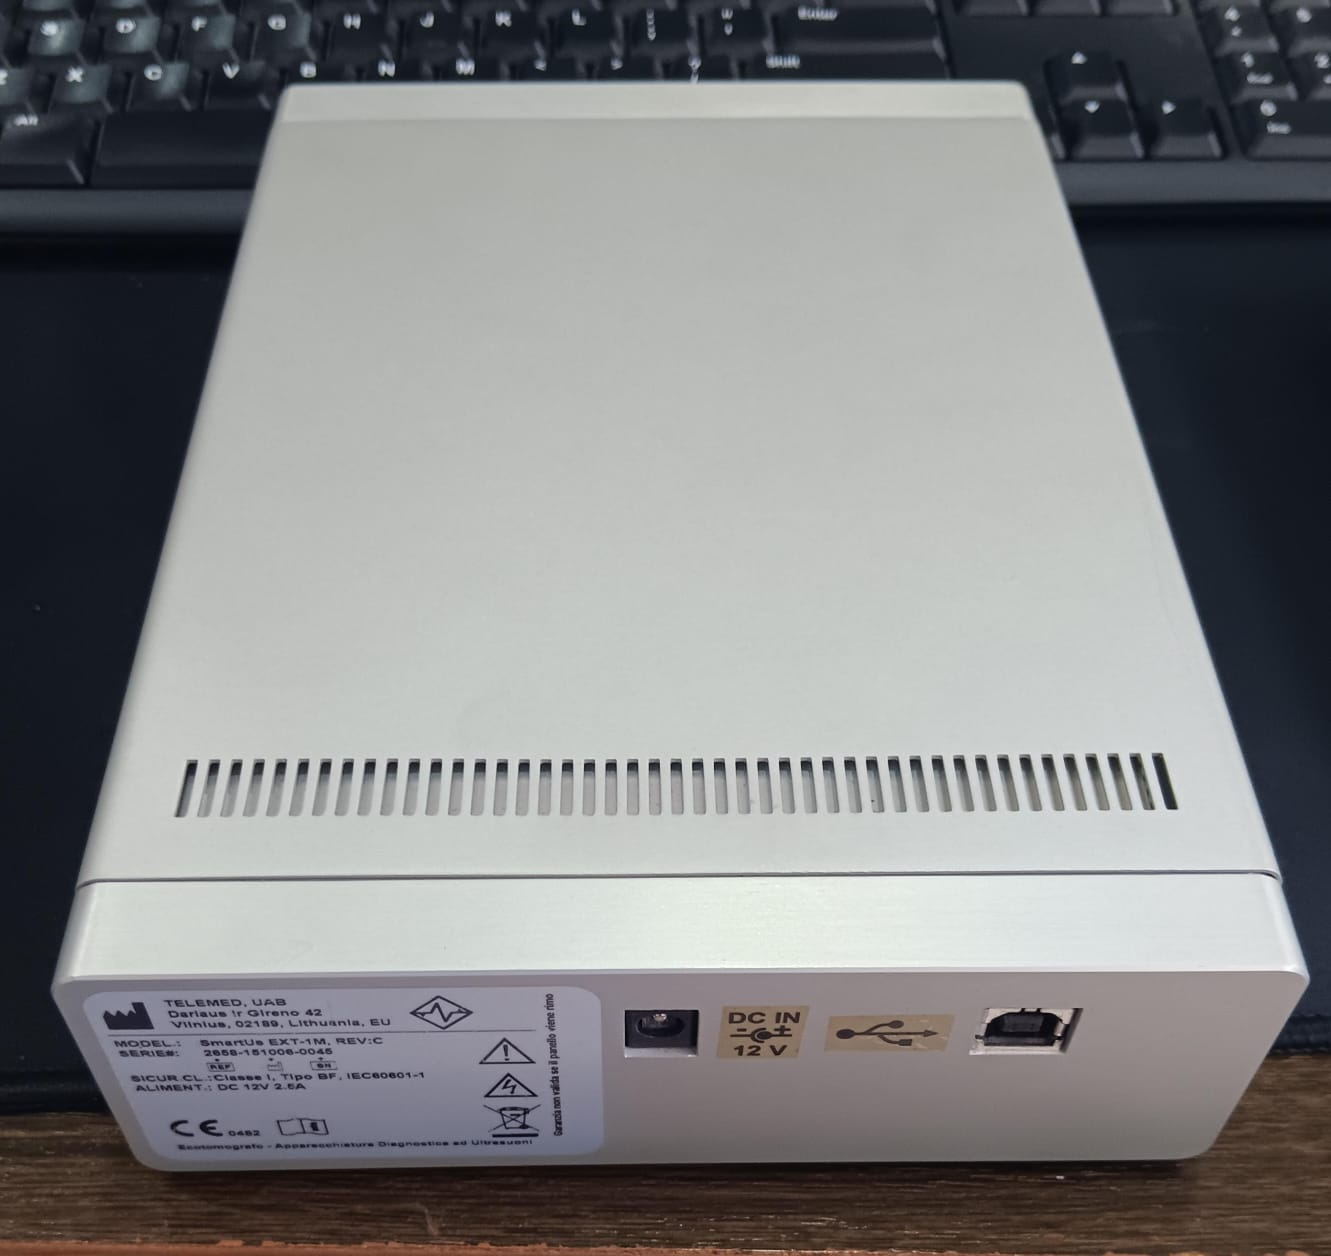
\includegraphics[scale=0.14]{bab3/usg_telemed.jpg}
		&
		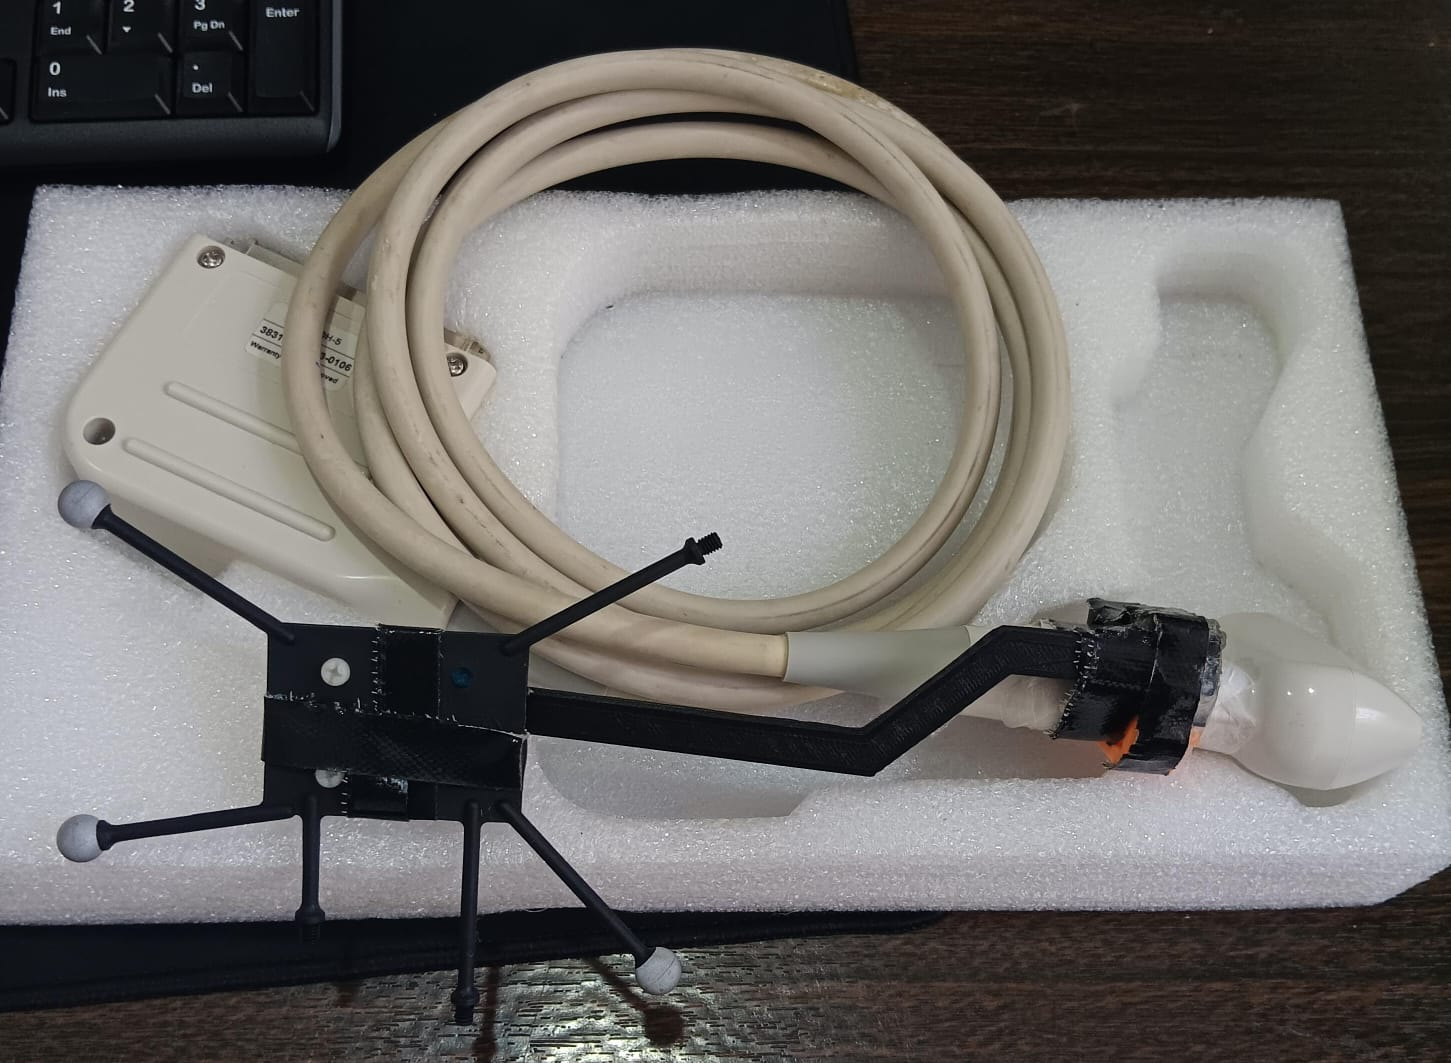
\includegraphics[scale=0.12]{bab3/probe_linear.jpg} \\
		\multicolumn{1}{c}{(a)} & \multicolumn{1}{c}{(b)} 
		
	\end{tabular}
	
	\begin{tabular}{ll}
		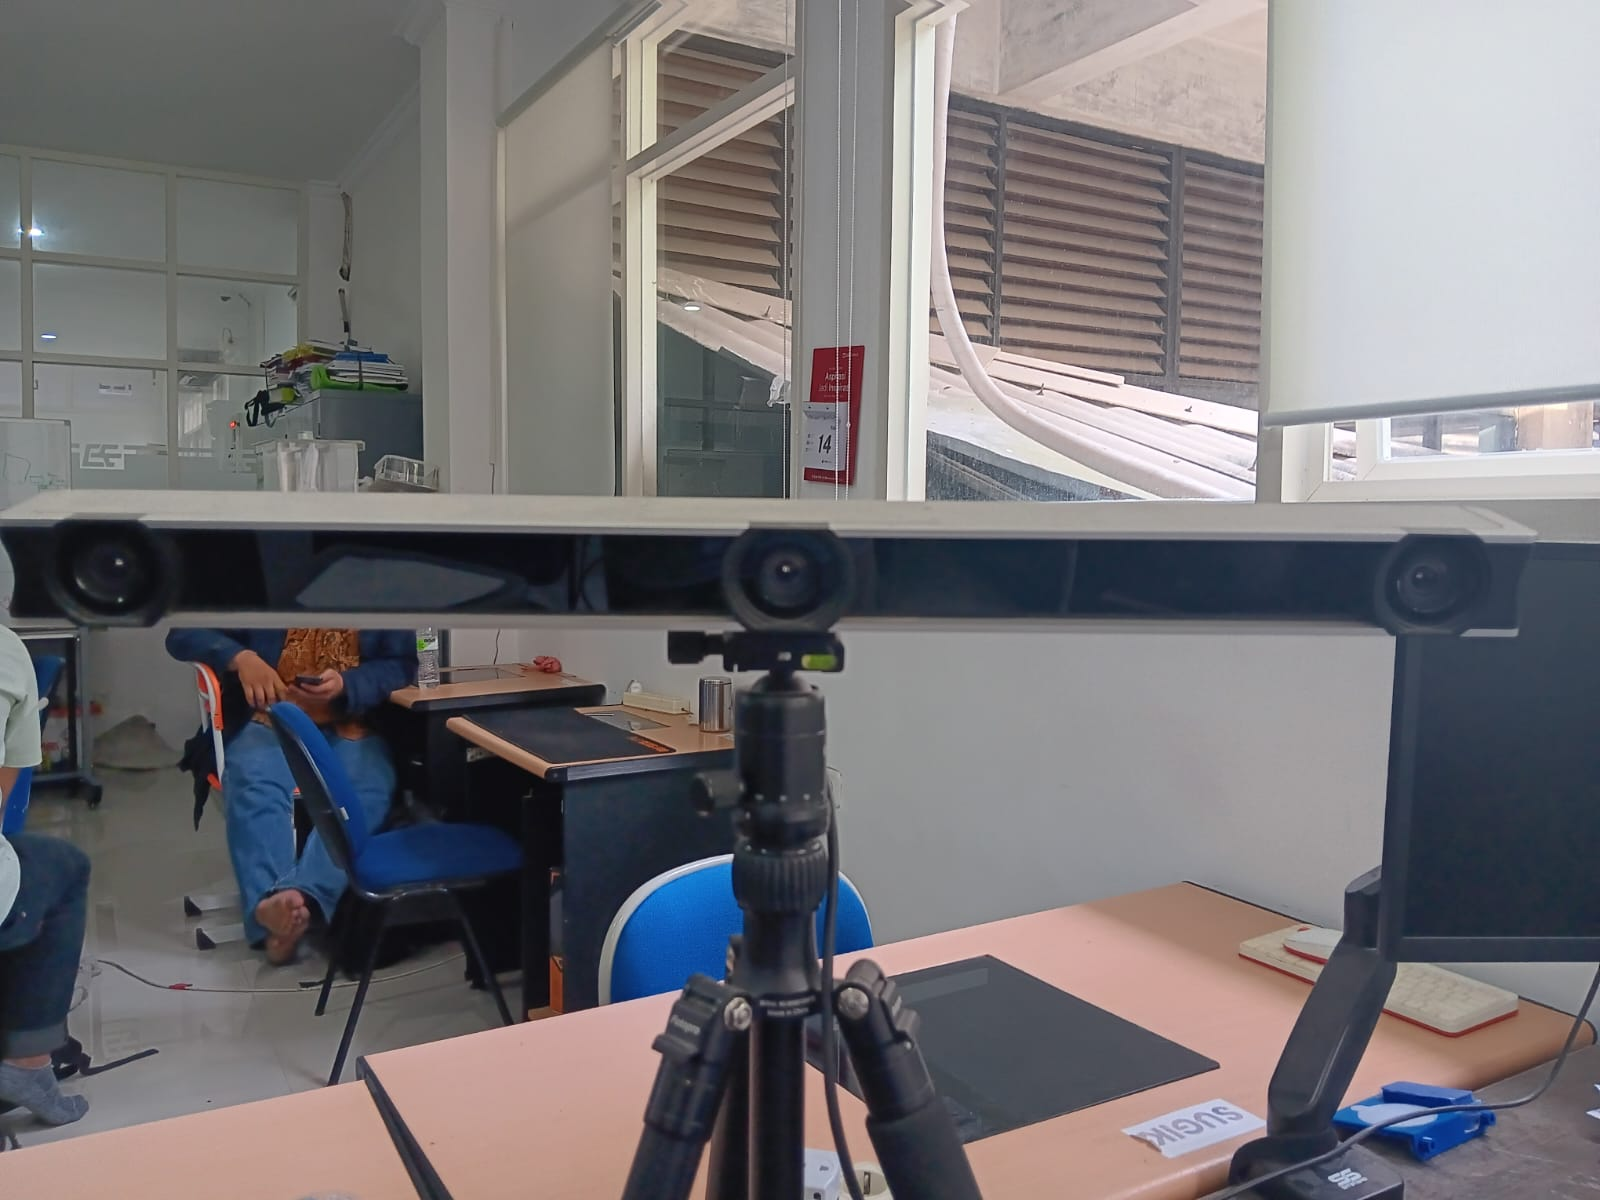
\includegraphics[scale=0.12]{bab3/img_optic_track.jpg}\\
		\multicolumn{1}{c}{(c)}  
		
	\end{tabular}
	\caption{(a) modalitas \textit{ultrasound} Telemed SmartUs EXT-1M, (b) Probe Linear, dan (c) perangkat \textit{OpticTrack V120:Trio}}
	\label{Fig:tools_data_acquition}
\end{figure}





\subsection{Prosedur Akuisisi Citra \textit{Ultrasound} Pembuluh Darah dan Gumpalan Darah Vena}
Prosedur akuisisi citra \textit{ultrasound} pembuluh darah dan gumpalan darah (\textit{thrombus}) vena membutuhkan perangkat  seperti \textit{probe} yang sudah terpasang marker, kamera \textit{optic track}, \textit{PC} yang digunakan untuk memproses dan memvisualkan citra, serta \textit{phantom} balon panjang. Akuisisi citra \textit{ultrasound thrombus} dilakukan dengan cara menempelkan permukaan \textit{probe} pada permukaan \textit{phantom} balon panjang. Fitur dan citra \textit{ultrasound thrombus} ditransformasikan ke dalam sistem koordinat marker yang terpasang pada pangkal \textit{probe} dan selanjutnya ditransformasikan ke dalam sistem koordinat kamera \textit{optic track} yang menjadi sistem koordinat global. Transformasi tersebut diperoleh dari hasil perhitungan jarak antara \textit{optic track} ke marker dan marker ke \textit{optic track}. 

%Konsep akuisisi data citra \textit{ultrasound} pembuluh darah dan \textit{thrombus} \textit{phantom} balon panjang dapat dilihat pada Gambar \ref{fig:prosedur_akuisisi}.
%
%\begin{figure}[H]
%	\centering
%	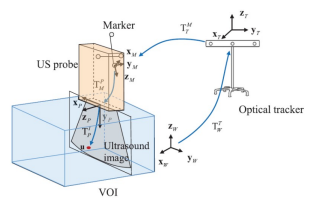
\includegraphics[scale= 0.7]{bab3/konsep_akuisisi_citra.png}
%	\caption{Konsep akuisisi data citra \textit{ultrasound} pembuluh darah dan \textit{thrombus} \textit{phantom} balon panjang}
%	\label{fig:prosedur_akuisisi}
%\end{figure}

Dalam proses akuisisi data menggunakan perangkat lunak dari hasil penelitian yang telah dilakukan sebelumnya. Perangkat lunak ini memiliki kemampuan untuk menyesuaikan tingkat kecerahan citra yang diperoleh, dapat mengatur frekuensi, kedalaman, dan titik fokus dari \textit{ultrasound}. Adapun antarmuka perangkat lunak yang digunakan untuk akuisisi citra 2D \textit{ultrasound thrombus} dapat dilihat pada Gambar. Proses akuisisi data menghasilkan citra 2D \textit{thrombus} pada pembuluh darah vena dengan dimensi 661 x 512 \textit{pixels} beserta data posisi marker yang berekstensi (\textit{.txt}). 


%Sebelum melakukan akuisisi citra, peneliti memastikan posisi marker yang terpasang pada pangkal \textit{probe} harus berhadapan dengan kamera \textit{optic track}. Hal itu bertujuan untuk memperoleh data posisi dari marker yang terpasang pada \textit{probe}. Data posisi marker diperoleh dari perhitungan jarak antara kamera \textit{optic track} ke marker dan marker ke kamera \textit{optic track}.    

% \subsection{Citra \textit{Ultrasound} Gumpalan Darah Vena}
% Data 2D citra USG gumpalan darah vena diperoleh dari data gumpalan darah lima pasien penderita DVT dengan total 317 citra. Gumpalan darah pasien terbentuk di dalam pembuluh darah vena bagian kaki. Data gumpalan darah ini menyajikan informasi visual yang dihasilkan dari pemindaian menggunakan sensor ultrasonografi (USG) yang memperlihatkan lokasi dan karakteristik gumpalan darah dalam pembuluh darah vena pada ke lima pasien tersebut. Data gumpalan darah ini penting untuk dianalisis guna membantu dokter dalam mendiagnosa, penilaian resiko, serta pengembangan metode pengobatan dan tindak lanjut untuk pasien penderita DVT.
% \begin{figure}[H]
% 	\centering
% 	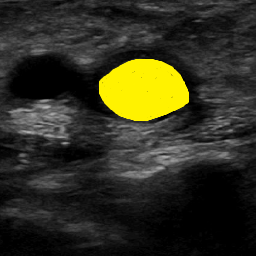
\includegraphics[scale= 0.7]{bab3/thrombus.png}
% 	\caption{Data Citra Ultrasound Gumpalan Darah}
% 	\label{fig:gumpalandarah}
% \end{figure}
%menggunakan peralatan seperti phantom, USG Telemed-SmartUs, dan Optitrack. Dalam proses pengambilan citra USG ini dilakukan dengan aturan dan ketentuan yang berlaku sebelum melakukan tahapan preprocessing.
%\subsection{Alat Pengambilan Citra}
%Penelitian ini menggunakan data ultrasound 2D gumpalan darah vena. Data citra gumpalan darah vena dikuisisi dari phantom yang merupakan replika dari bagian tubuh manusia. Phantom berbentuk gumpalan daging yang di dalamnya terdapat pembuluh darah beserta gumpalan darahnya. Pada penelitian ini Phantom akan menjadi sumber data utama simulasi gumpalan darah vena. Adapun phantom yang digunakan pada penelitian ini dapat dilihat pada Gambar 3.2.
%
%\begin{figure}[H]
%	\centering
%	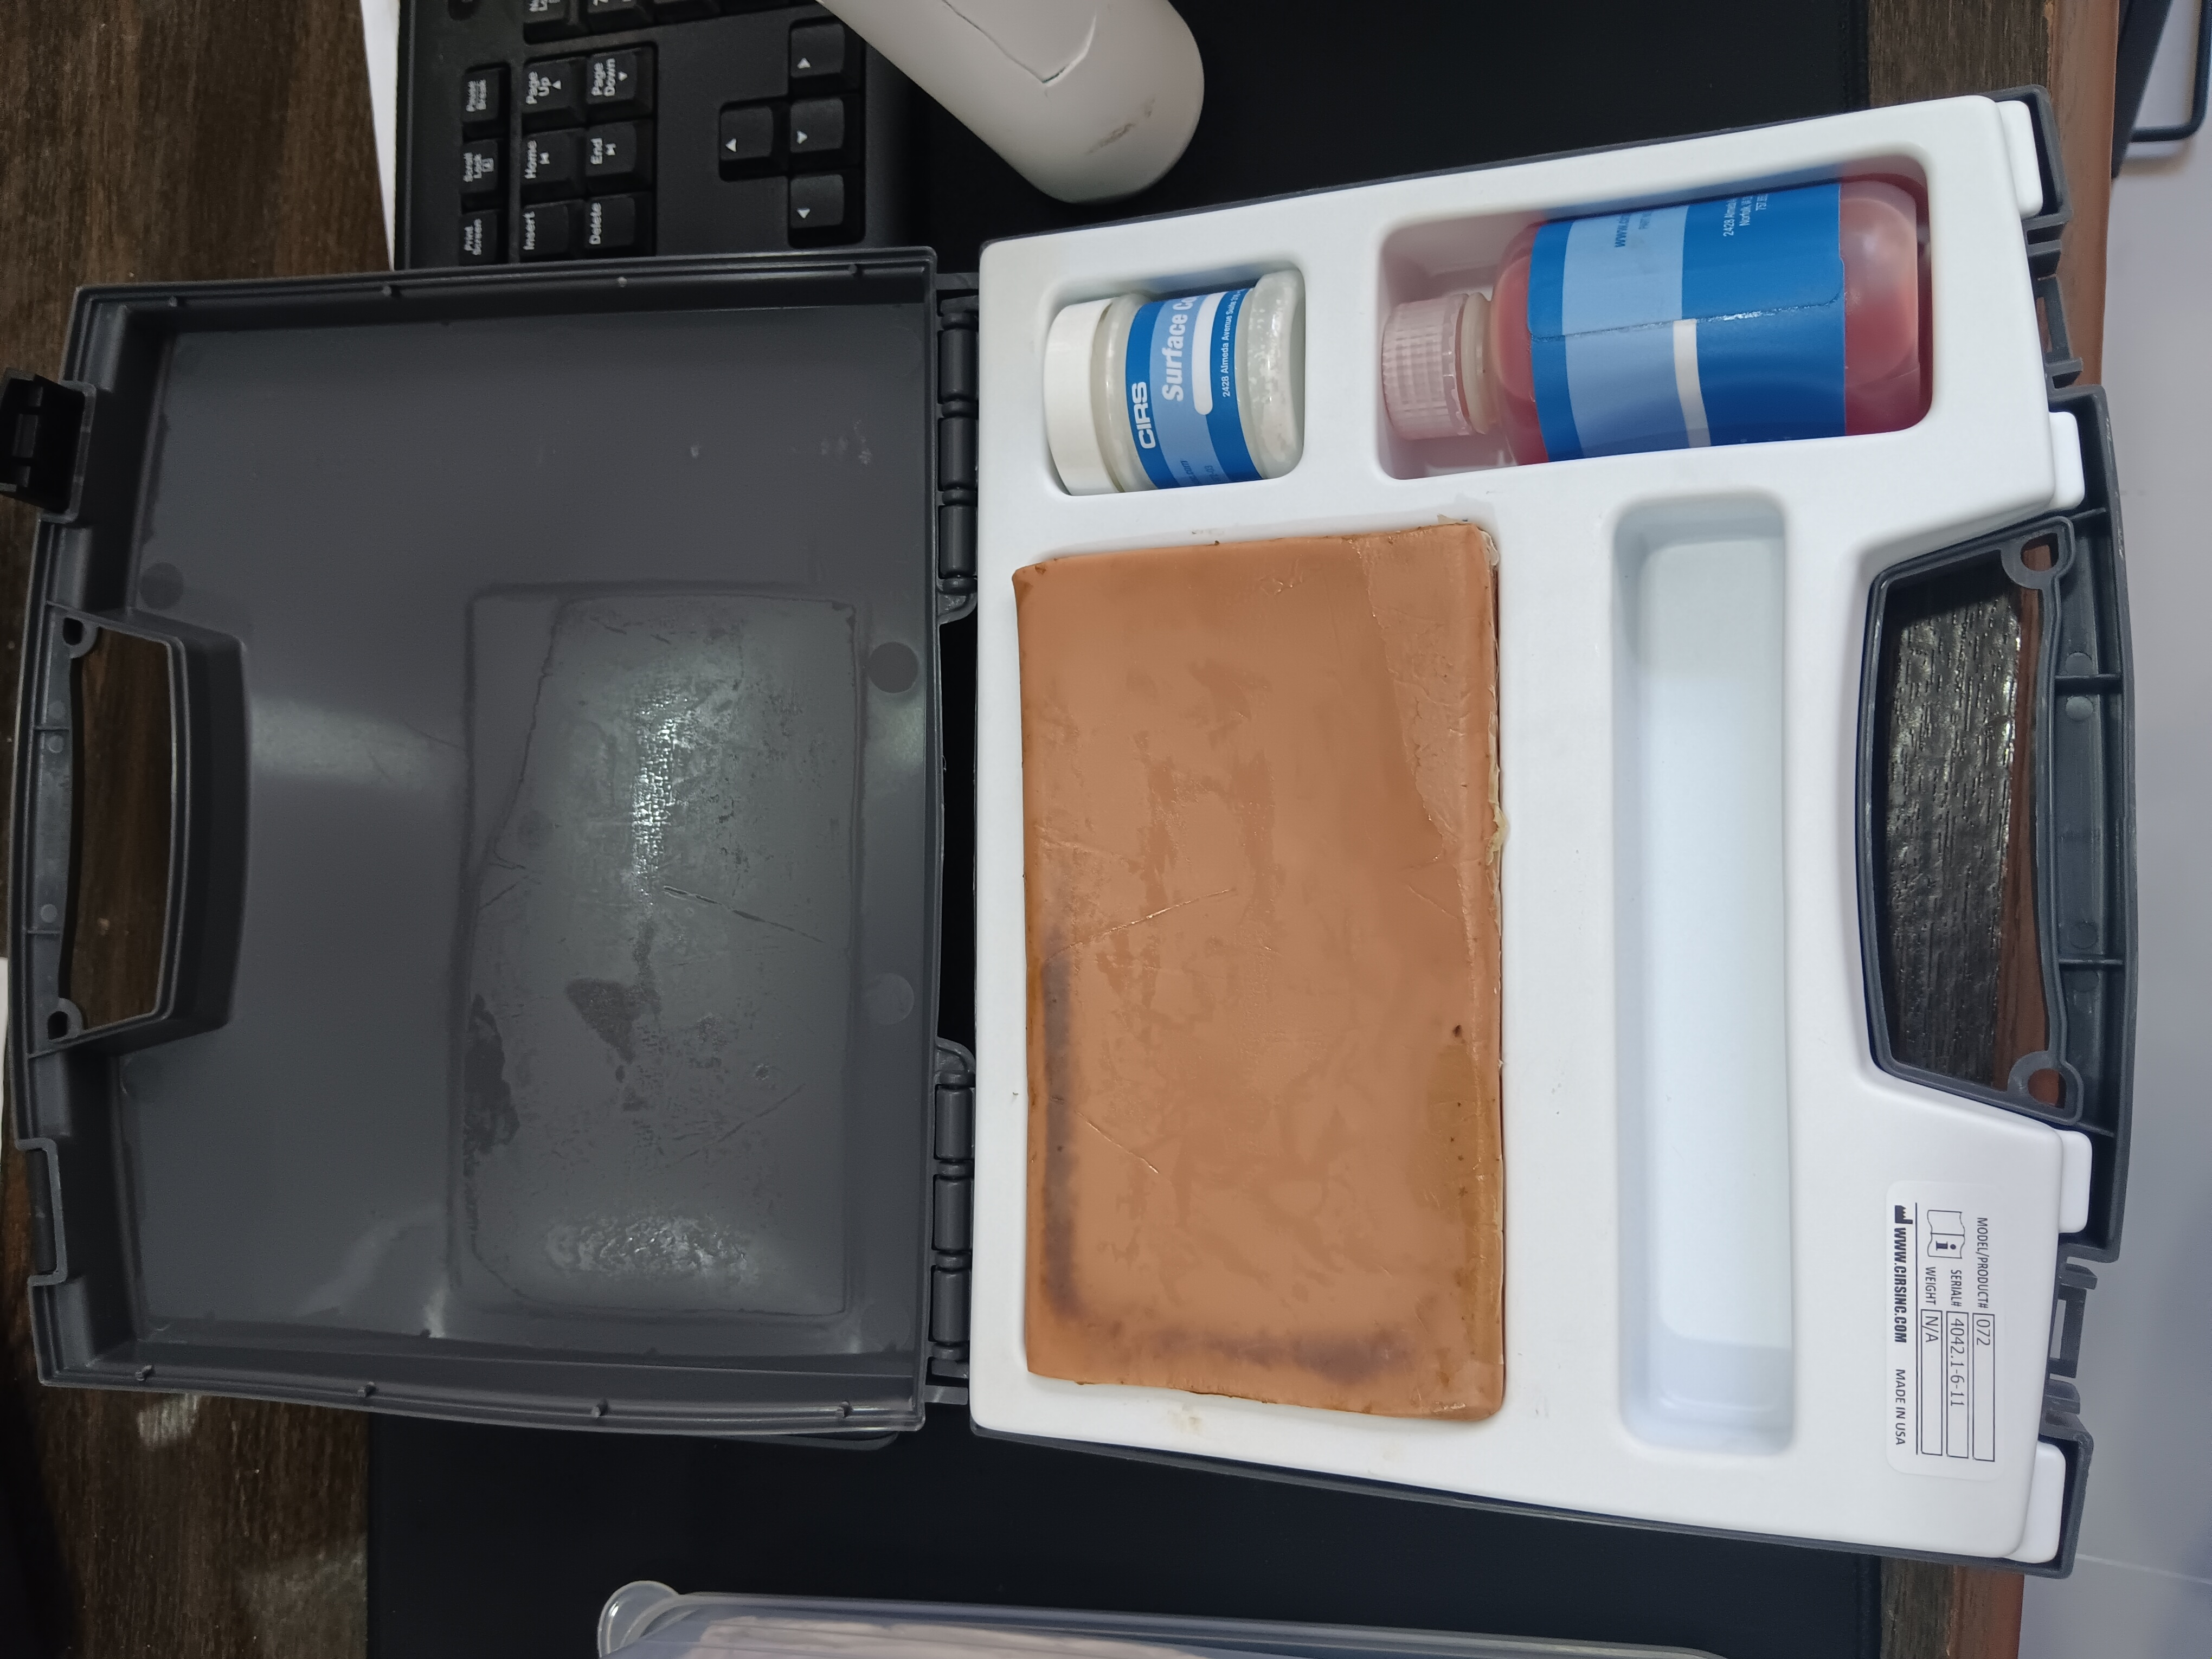
\includegraphics[width=\linewidth, angle=-90]{bab3/phantom.jpg}
%	\caption{Phantom}
%	\label{fig:phantom}
%\end{figure}
%
%Selain menggunakan phantom sebagai sumber data penelitian, peneliti akan menggunakan data gumpalan darah vena penderita DVT. Hal itu dilakukan agar dataset yang digunakan dalam proses pelatihan menggunakan model deep learning V-Net menjadi lebih bervariasi serta diharapkan mendapatkan hasil segmentasi area gumpalan darah vena yang akurat. 
%%adalah citra yang diperoleh dari kamera dengan ukuran $300\times 300$ dari beberapa sudut pandang yang berlainan.
%\subsection{Proses Pengambilan Citra}
\section{Preprocessing}
Citra 2D gumpalan darah (\textit{thrombus}) yang telah diakuisisi akan melalui dua langkah utama dalam tahap {\textit{preprocessing} sebelum masuk ke dalam proses \textit{training} menggunakan model \textit{deep learning} U-Net. Adapun tahap \textit{preprocessing} terbagi menjadi dua tahap yaitu rekonstruksi 3D citra \textit{ultrasound thrombus} dan mereduksi \textit{noise}. 
	
%normalisasi citra 2D \textit{ultrasound thrombus} dan mengubah bentuk 2D menjadi citra 3D \textit{thrombus}.

\subsection{Rekonstruksi 3D Citra \textit{Ultrasound} Pembuluh Darah dan Gumpalan Darah Vena}
\subsubsection{Penempatan Citra 2D \textit{Ultrasound} Pembuluh Darah dan Gumpalan Darah Vena pada Ruang \textit{Voxel} 3D}

%Penempatan setiap piksel citra \textit{ultrasound} pebuluh darah dan gumpalan darah \textit{thrombus} pada ruang \textit{voxel} 3D didasari oleh transformasi yang diperoleh pada proses kalibrasi. Ukuran ruang \textit{voxel} 3D ditentukan dengan cara mencari nilai batas nilai minimum dan nilai maksimum pada koordinat x,y, dan z. Batas tersebut didasari oleh posisi pada transformasi sistem koordinat pada ruang 3D.
Setelah dilakukan akuisisi data \textit{ultrasound} pembuluh darah dan gumpalan darah (\textit{thrombus}) \textit{phantom} balon panjang, setiap piksel citra tersebut ditempatkan pada ruang \textit{voxel} 3D berdasarkan transformasi yang diperoleh pada proses kalibrasi. Sebelum ditempatkan pada ruang \textit{voxel} 3D, harus dilakukan pembentukan ruang \textit{voxel} 3D terlebih dahulu. Proses pembuatan ruang \textit{voxel} disesuaikan dengan ukuran ruang \textit{voxel} yang dibutuhkan untuk penempatan hasil transformasi setiap citra \textit{ultrasound} pembuluh darah dan \textit{thrombus} \textit{phantom} balon panjang. Setiap piksel pada citra \textit{ultrasound} pembuluh darah dan \textit{thrombus} \textit{phantom} balon panjang ($f(u,v)$) dengan ukuran baris ($m$) dan kolom ($n$) akan ditempatkan pada voksel ($V(x,y,z)$). Adapun gambaran tentang penempatan citra \textit{ultrasound} pembuluh darah dan \textit{thrombus} \textit{phantom} balon panjang dapat dilihat pada Gambar \ref{fig:visualisasi_penempatan_voxel3d}. 

\begin{figure}[htbp]
	\centering
	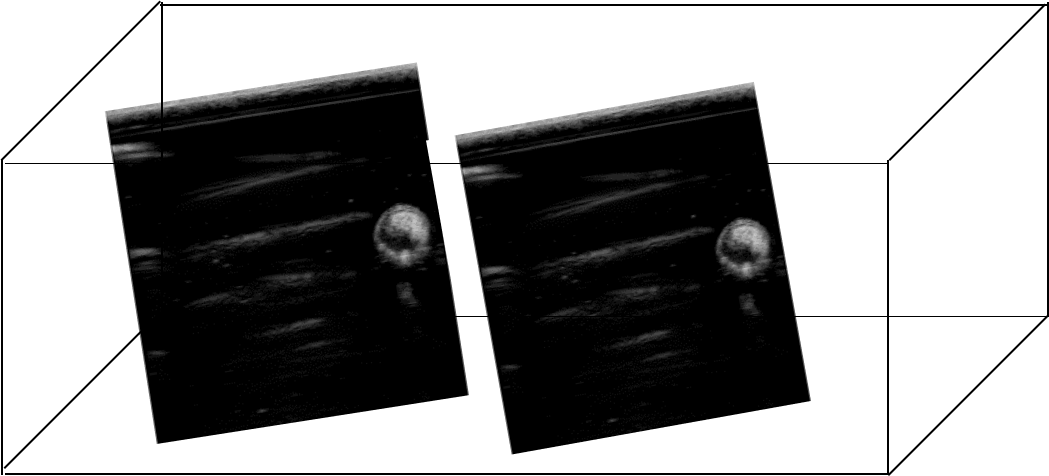
\includegraphics[scale= 0.3]{bab3/visualisasi_penempatan_voxel_3d.png}
	\caption{Visualisasi Penempatan Voxel 3D}
	\label{fig:visualisasi_penempatan_voxel3d}
\end{figure}

Adapun proses penempatan setiap piksel citra \textit{ultrasound} pada ruang \textit{voxel} 3D berdasarkan transformasi yang diperoleh pada proses kalibrasi dapat dirumuskan dengan Persamaan \ref{eq:transformasi-citra2d3d}. 

\begin{equation}
	\label{eq:transformasi-citra2d3d}
	V(x,y,z)\ =\ {_P^T}T\ \times{_U^P}T\ \ \times \begin{pmatrix}u \\v \\0 \\1\end{pmatrix}\
\end{equation}


Berdasarkan persamaan \ref{eq:transformasi-citra2d3d}, variabel \textit{V(x,y,z)} merupakan posisi \textit{voxel} yang merepresentasikan posisi data citra dalam ruang 3D. Variabel $_{P}^{T}T$  merupakan transformasi dari marker pada probe ultrasound ke pusat koordinat sistem kamera \textit{optictrack}. Variabel $_{U}^{P}T$  merupakan transformasi dari bidang citra \textit{ultrasound} ke marker pada \textit{probe ultrasound}. Variabel \textit{u} dan \textit{v} merupakan koordinat \textit{pixel} dari citra 2D. Adapun bagan proses penempatan piksel citra 2D \textit{ultrasound} pembuluh darah dan \textit{thrombus} \textit{phantom} balon panjang pada ruang \textit{voxel} 3D dengan kamera \textit{optic track} dapat dilihat pada Gambar \ref{fig:prosedur_rekonstruksi}.


\begin{figure}[htbp]
	\centering
	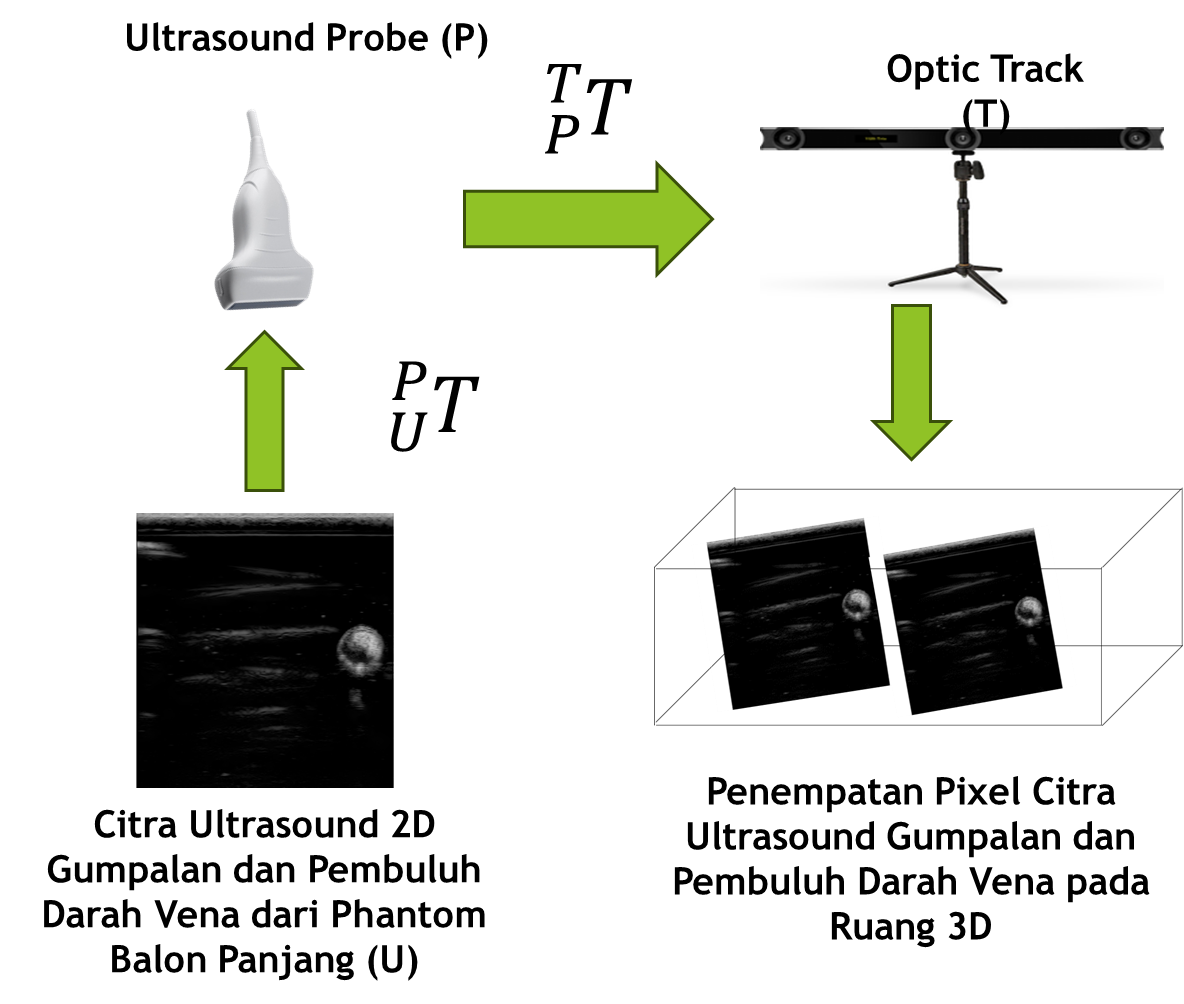
\includegraphics[scale= 0.25]{bab3/prosedur_rekonstruksi.png}
	\caption{Prosedur Rekonstruksi 3D}
	\label{fig:prosedur_rekonstruksi}
\end{figure}

Visualisasi hasil rekonstruksi 3D pada citra \textit{ultrasound} pembuluh darah dan \textit{thrombus} \textit{phantom} balon panjang menggunakan perangkat lunak \textit{3D slicer}. Hasil visualisasi tersebut dapat dilihat pada Gambar \ref{fig:visualisasi_hasil_rekosntruksi}.

\begin{figure}[htbp]
	\centering
	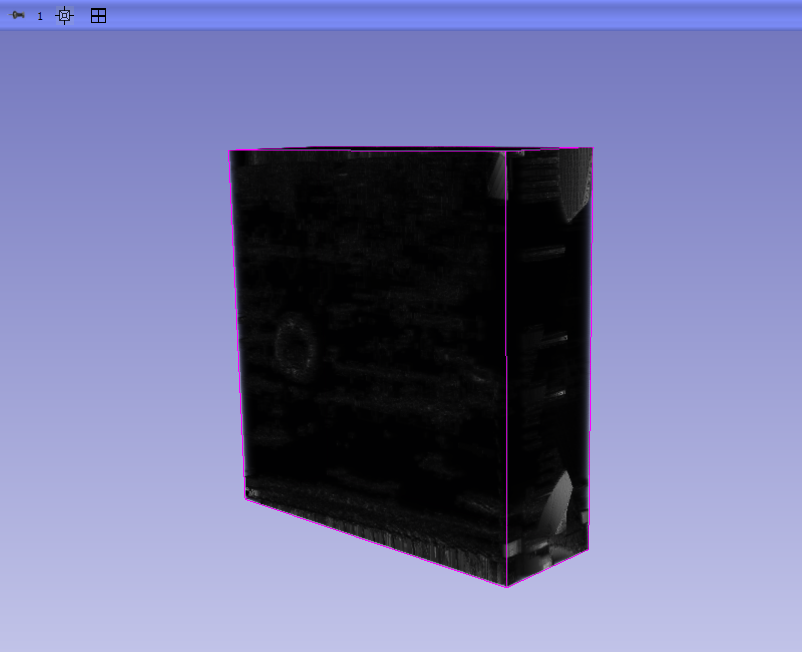
\includegraphics[scale= 0.5]{bab3/Hasil_Rekonstruksi_3d.png}
	\caption{Visualisasi hasil rekonstruksi 3D citra \textit{ultrasound} pembuluh darah dan \textit{thrombus} \textit{phantom} balon panjang menggunakan perangkat lunak \textit{3D Slicer}.}
	\label{fig:visualisasi_hasil_rekosntruksi}
\end{figure}




%\subsubsection{Visualisasi Hasil Rekonstruksi 3D Citra \textit{Ultrasound} Pembuluh Darah dan Gumpalan Darah Vena}


\subsection{Reduksi \textit{Noise}}
Pada penelitian ini data yang digunakan adalah data citra 3D \textit{ultrasound} pembuluh darah dan gumpalan darah (\textit{thrombus}) dari hasil rekonstruksi 3D serta data citra 2D \textit{ultrasound} \textit{thrombus} pada pembuluh darah vena penderita DVT (\textit{Deep Vein Thrombosis}). Citra \textit{ultrasound} \textit{thrombus} memiliki tingkat \textit{noise} yang tinggi. Oleh karena itu citra \textit{ultrasound thrombus} akan melalui tahap reduksi \textit{noise}. Khusus untuk citra 3D \textit{ultrasound} pembuluh darah dan gumpalan darah (\textit{thrombus}) dari hasil rekonstruksi 3D, agar mempermudah proses reduksi \textit{noise}, citra 3D tersebut di \textit{slice} menjadi citra 2D terlebih dahulu. Filter \textit{denoising} yang digunakan dalam penelitian ini yaitu filter \textit{gaussian}, filter \textit{median}, filter \textit{mean}, filter \textit{bilateral}, dan filter \textit{non local means}. Alasan peneliti memilih 5 filter \textit{denoising} tersebut dikarenakan ke lima filter \textit{denoising} tersebut sering digunakan dalam proses reduksi \textit{noise} citra biomedis. Filter \textit{gaussian} merupakan sebuah teknik dalam pengolahan citra yang digunakan untuk menghaluskan atau mengaburkan citra. Hal itu bertujuan untuk mengurangi detail - detail yang tidak diinginkan seperti \textit{noise} dalam sebuah citra. 
Filter \textit{gaussian} menggunakan operasi konvolusi, yaitu sebuah proses matematis dimana dapat menggabungkan 2 informasi. Informasi tersebut ialah citra asli dan sebuah matriks kernel. Kernel ini memiliki nilai - nilai tertentu yang membantu dalam reduksi \textit{noise}. Adapun filter \textit{gaussian} direpresentasikan dalam Persamaan \ref{eq:rumus_gaussian}.

\begin{equation}
	G\left(x,y\right)=\ e^\frac{{x^2+y}^2}{2\sigma^2}
	\label{eq:rumus_gaussian}
\end{equation}

Variabel $G(x,y)$ menunjukkan nilai filter \textit{gaussian} pada koordinat $(x,y)$ dalam ruang 2 dimensi. Variabel $e$ menunjukkan simpangan baku dari distribusi tersebut. Filter kedua yang digunakan dalam penelitian ini yaitu filter \textit{median}. Filter median merupakan salah satu filter yang paling umum digunakan dalam dunia biomedik. Operasi pada filter \textit{median} sangat sederhana yaitu dengan cara menggantikan nilai piksel tengah dengan nilai median dari piksel tetangganya. Perhitungan untuk mendapatkan hasil filter \textit{median} dapat dilihat pada Persamaan \ref{eq:rumus_median}.

\begin{equation}
	A(x,y) = median\left\{ f\left( x - i, y - i \right),i,j\in W  \right\}
	\label{eq:rumus_median}
\end{equation}

Dimana, variabel $W$ menunjukkan citra mask 2D, variabel $A(x,y)$ menunjukkan hasil output citra, dan variabel $f(x,y)$ menunjukkan citra asli. Filter ketiga yang digunakan dalam penelitian ini yaitu filter \textit{mean}. Filter \textit{mean} berfungsi untuk mengurangi \textit{noise} serta menghaluskan citra dengan memanfaatkan jumlah variasi intensitas minimal antara piksel yang berdekatan. Adapun filter \textit{mean} dapat dilihat pada Persamaan \ref{eq:rumus_mean}.

\begin{equation}
	f(x,y) = \frac{1}{mn}\sum_{(s,t)\epsilon S_{xy}}g(s,t)
	\label{eq:rumus_mean}
\end{equation}

Variable $f(x,y)$ menunjukkan nilai piksel hasil setelah proses penghalusan pada koordinat $(x,y)$ menggunakan filter \textit{mean}. Variabel $m$ dan $n$ menunjukkan jumlah baris dan kolom pada kernel. Variabel $g(s,t)$ menunjukkan nilai piksel pada koordinat $(s,t)$ sebelum penghalusan. Simbol sigma $\sum$ menunjukkan penjumlahan semua nilai piksel $g(s,t)$ di dalam kernel $S_{x,y}$. Filter yang keempat yan digunakan dalam penelitian ini yaitu filter \textit{bilateral}. Filter reduksi \textit{noise} \textit{bilateral} mempertimbangkan intensitas piksel berdasarkan lokasi piksel target maupun perbedaan jarak antar piksel. Berdasarkan hal tersebut, filter \textit{bilateral} efektif dalam mengurangi \textit{noise} citra tanpa mengaburkan tepi dan detail penting dalam citra. Adapun filter \textit{bilateral} dapat dilihat pada Persamaan \ref{eq:rumus_bilateral_1}. 


\begin{equation}\label{eq:rumus_bilateral_1}
	\begin{split}
		&I^{filtered}(x) = \frac{1}{W_p}\sum_{x_i\in\Omega}I\left(x_i\right)f_r(\parallel I\left(x_i\right) - I\left(x\right)\parallel)\\&g_s(\parallel \left(x_i\right)-x \parallel)
	\end{split}
\end{equation}


\begin{equation}
	{W_p}=\sum_{x_i\in\Omega}f_r(\parallel I\left(x_i\right) - I\left(x\right)\parallel)g_s(\parallel \left(x_i\right)-x \parallel)
	\label{eq:rumus_bilateral_2}
\end{equation}

Dimana, $W_p$ merupakan normalisasi. Variabel $I^{filtered}$ merepresentasikan citra yang telah difilter. Variabel $x$ merepresentasikan koordinat dari piksel saat ini yang digunakan untuk difilter. Variabel $I$ mewakili citra asli. Variabel $f_r$ merepresentasikan perubahan kernel untuk intensitas penghalusan. Variabel $g_s$ menunjukkan kernel abstraksi untuk menghaluskan fluktuasi koordinat. Kemudian filter reduksi \textit{noise} yaitu filter \textit{non local means}. Filter \textit{denoising} ini dirancang untuk menjaga informasi citra sekaligus menghilangkan \textit{noise} pada citra. Adapun perhitungan filter \textit{non local means} dapat dilihat pada Persamaan \ref{eq:rumus_nlm}.

\begin{equation} \label{eq:rumus_nlm}
	\begin{split}
		&NLM\mid I(m)\mid =\sum_{n\epsilon N_m}\omega(N_m,\ N_n)I(n)\\ &\left(\omega(N_m,\ N_n) = \frac{1}{Z\left(m\right)^{\mathcal{e}^\frac{-d}{h^2}}}\right)
	\end{split}    
\end{equation}

Dimana, variabel $I(n)$ merepresentasikan intensitas \textit{noise}. Variabel $\omega(N_m,\ N_n)$ merepresentasikan jumlah perbedaan antara piksel target dan piksel sekitarnya. Variabel $Z(m)$ merepresentasikan konstanta  normalisasi. Serta variabel $d$ menunjukkan jarak \textit{euclidean}. Adapun hasil reduksi \textit{noise} citra \textit{ultrasound thrombus} dan pembuluh darah \textit{phantom} balon panjang dan citra \textit{thrombus} pasien penderita DVT dapat dilihat pada Gambar \ref{fig:hasil_denoising_rekonstruksi} dan Gambar \ref{fig:hasil_denoising_ori}.

\begin{figure}[htbp]
	\centering
	\begin{tabular}{ccc}
			% Baris pertama dengan tiga gambar
			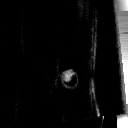
\includegraphics[width=0.3\textwidth]{bab3/reduksi_noise/img_360_ori.png} &
			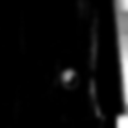
\includegraphics[width=0.3\textwidth]{bab3/reduksi_noise/img_360_gaussian.png} &
			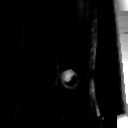
\includegraphics[width=0.3\textwidth]{bab3/reduksi_noise/img_360_median.png} \\
			(a)  & (b)  & (c)  \\ % Caption untuk baris pertama
			% Baris kedua dengan tiga gambar
			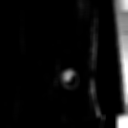
\includegraphics[width=0.3\textwidth]{bab3/reduksi_noise/img_360_mean.png} &
			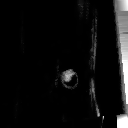
\includegraphics[width=0.3\textwidth]{bab3/reduksi_noise/img_360_bilateral.png} &
			
\includegraphics[width=0.3\textwidth]{bab3/reduksi_noise/img_360_nlm.png} \\
			(d)  & (e)  & (f)  % Caption untuk baris kedua
		\end{tabular}
	\caption{Hasil reduksi \textit{noise} citra \textit{ultrasound} pembuluh darah dan \textit{thrombus} \textit{phantom} balon panjang menggunakan filter sebagai berikut (a) tidak menggunakan filter; (b) filter \textit{gaussian}; (c) filter \textit{median}; (d) filter \textit{mean}; (e) filter \textit{bilateral}; (f) filter \textit{non-local means}}
	\label{fig:hasil_denoising_rekonstruksi}
\end{figure}


\begin{figure}[h]
	\centering
	\begin{tabular}{ccc}
		% Baris pertama dengan tiga gambar
		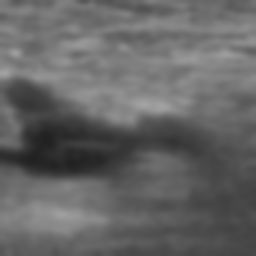
\includegraphics[width=0.3\textwidth]{bab4/citra-asli.jpg} &
		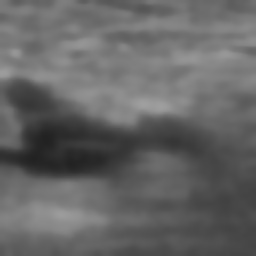
\includegraphics[width=0.3\textwidth]{bab4/citra-bilateral.jpg} &
		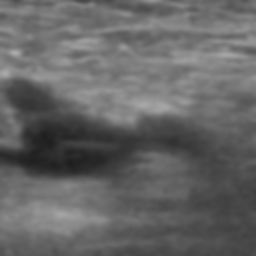
\includegraphics[width=0.3\textwidth]{bab4/citra-gaussian.jpg} \\
		(a)  & (b)  & (c)  \\ % Caption untuk baris pertama
		% Baris kedua dengan tiga gambar
		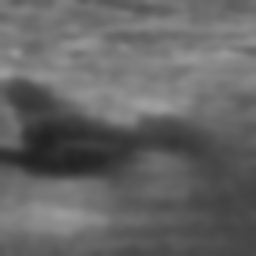
\includegraphics[width=0.3\textwidth]{bab4/citra-mean.jpg} &
		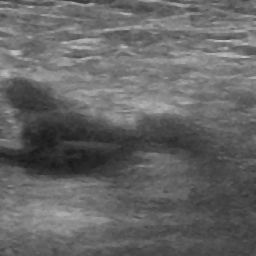
\includegraphics[width=0.3\textwidth]{bab4/citra-median.jpg} &
		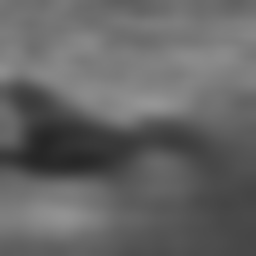
\includegraphics[width=0.3\textwidth]{bab4/citra-nlm.jpg} \\
		(d)  & (e)  & (f)  % Caption untuk baris kedua
	\end{tabular}
	\caption{Hasil reduksi \textit{noise} citra \textit{ultrasound} \textit{phantom} balon panjang menggunakan filter sebagai berikut (a) tidak menggunakan filter; (b) filter \textit{bilateral}; (c) filter \textit{gaussian}; (d) filter \textit{mean}; (e) filter \textit{median}; (f) filter \textit{non-local means}}
	\label{fig:hasil_denoising_ori}
\end{figure}

Citra 2D \textit{ultrasound} pembuluh darah dan \textit{thrombus} yang telah melalui tahapan reduksi \textit{noise} akan dilakukan pembuatan \textit{groundtruth} dengan menggunakan perangkat lunak \textit{Label Studio}. Perangkat lunak \textit{Label Studio} bersifat \textit{open source} yang tersedia melalui \textit{Python Package Index} (PyPI). Alasan peneliti memilih perangkat lunak \textit{Label Studio} karena perangkat lunak \textit{open source} ini dapat dioperasikan secara lokal dan mendukung berbagai jenis model anotasi dengan output yang diinginkan. Proses \textit{labelling} pada citra \textit{ultrasound} 2D ini menggunakan anotasi masking area untuk dua kelas yaitu \textit{multiclass semantic segmentation}. Metode ini menghasilkan citra hitam putih dimana area pembuluh darah vena dan \textit{thrombus} ditandai denga warna putih. Sementara itu, area lain yang diinterpretasikan sebagai bukan area pembuluh darah vena dan \textit{thrombus} ditandai dengan warna hitam.Citra hasil anotasi biasa disebut dengan citra \textit{mask}. Citra \textit{mask} ini kemudian diunduh dalam format file .PNG. Adapun proses pembuatan citra \textit{mask} dapat dilihat pada Gambar \ref{fig:label-studio}.

\begin{figure}[htbp]
	\centering
	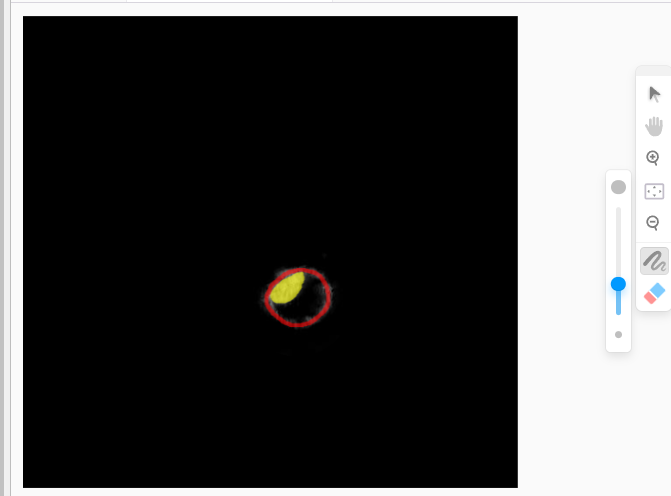
\includegraphics[scale= 0.25]{bab3/label-studio.png}
	\caption{Proses Pembuatan Citra Mask Menggunakan \textit{Label Studio}}
	\label{fig:label-studio}
\end{figure}

\begin{figure}[htbp]
	\centering
	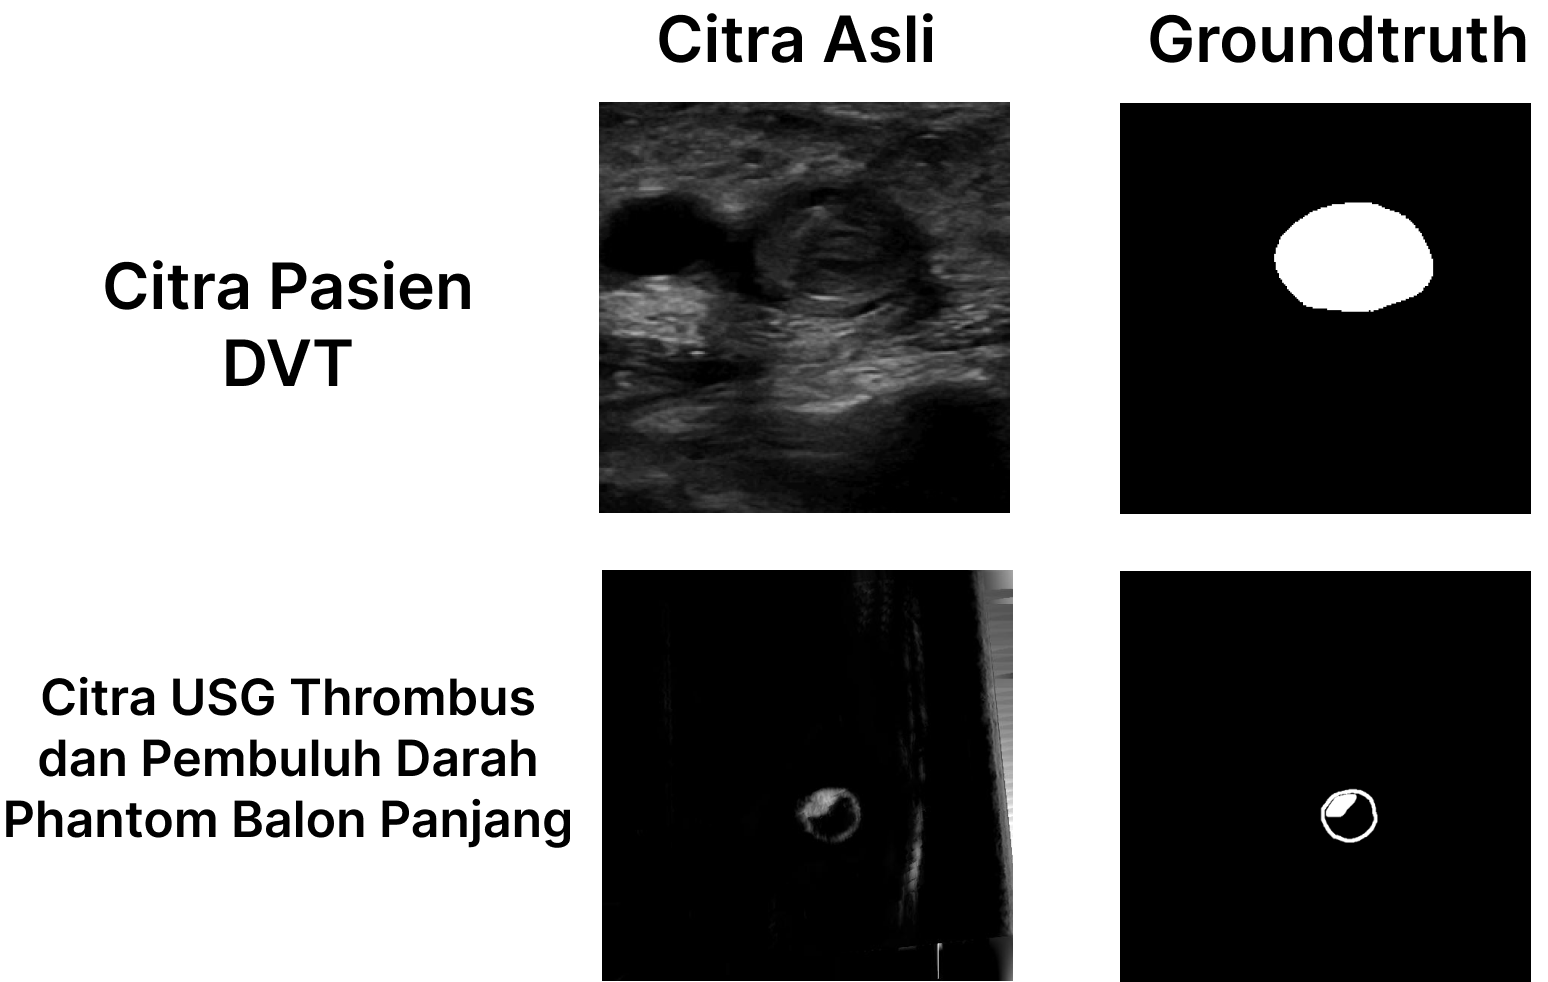
\includegraphics[scale= 0.15]{bab3/Hasil-Label.png}
	\caption{Proses Pembuatan Citra Mask Menggunakan \textit{Label Studio}}
	\label{fig:result-label}
\end{figure}

%Citra pembuluh darah dan gumpalan darah \textit{thrombus} yang telah direkonstruksi menjadi bentuk 3D, seringkali mengandung \textit{noise} yang tinggi yang dapat mengganggu interpretasi dan analisis lebih lanjut. Oleh karena itu, citra 3D akan diubah menjadi citra 2D melalui proses \textit{slicing} untuk mempermudah dalam proses reduksi \textit{noise}.
%
%Proses reduksi \textit{noise} pada citra \textit{ultrasound} pembuluh darah dan \textit{thrombus} ini sangat penting. Keberadaan \textit{noise} dapat menyebabkan kesalahan dalam menginterpretasi citra dan mempengaruhi keakuratan diagnosa. Langkah pertama pada proses reduksi \textit{noise} pada citra \textit{ultrasound} pembuluh darah dan \textit{thrombus} hasil rekonstruksi yaitu menggunakan teknik \textit{Hough Transform} yang merupakan sebuah metode dalam OpenCV yang efektif untuk mendeteksi bentuk geometris berupa lingkaran. \textit{Hough Transform} digunakan untuk mengidentifikasi dan menandai area dalam citra \textit{ultrasound} yang sesuai dengan bentuk lingkaran. Bentuk lingkaran merupakan karakteristik dari pembuluh darah pada citra.
%
%Setelah berhasil mengidentifikasi lingkaran menggunakan metode \textit{Hough Transform}, langkah berikutnya yaitu memisahkan objek lingkaran beserta objek yang berada di dalam radius lingkaran tersebut dari bagian lainnya dalam citra. Hal ini dilakukan dengan cara menggelapkan area di sekitar lingkaran, yaitu dengan membuat bagian luar dari radius lingkaran menjadi hitam. Langkah ini membantu dalam meningkatkan fokus pada area pembuluh darah dan \textit{thrombus}, sekaligus menghilangkan elemen - elemen lain yang menambah \textit{noise} pada citra. Dengan demikian, proses ini tidak hanya mengurangi \textit{noise} tetapi juga dapat memudahkan analisis dan interpretasi citra \textit{ultrasound} pembuluh darah dan \textit{thrombus} dengan lebih jelas dan akurat. Adapun hasil reduksi noise dapat dilihat pada Gambar \ref{fig:comparison-denoising}.
%
%
%\begin{figure}[htbp]
%	\centering
%	\begin{tabular}{ccc}
%		\textbf{Citra Asli} & \textbf{Denoising} \\
%		% Baris pertama dengan tiga gambar
%		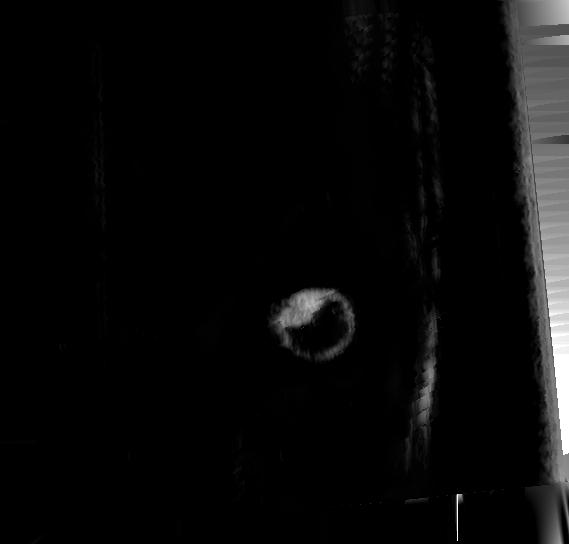
\includegraphics[scale=0.3]{bab3/citra-asli-rekonstruksi.jpg} &
%		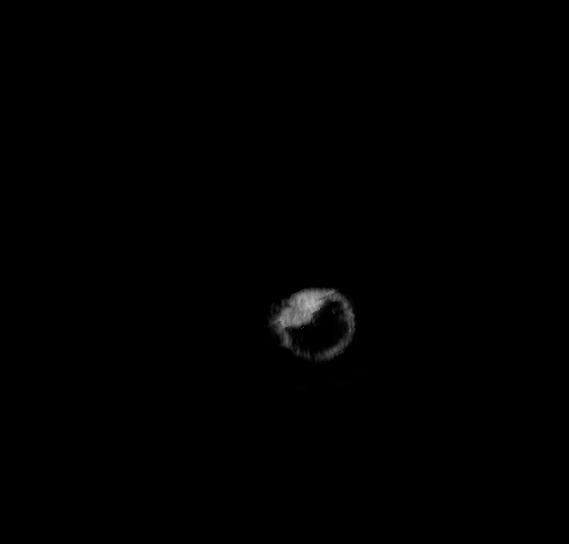
\includegraphics[scale=0.3]{bab3/citra-asli-denoising-rekonstruksi.png} & \\
%		(a) & (b)    % Caption untuk baris pertama
%		% Caption untuk baris kedua
%	\end{tabular}
%	\caption{(a) Citra asli dan (b) Citra hasil \textit{denoising}}
%	\label{fig:comparison-denoising}
%\end{figure}  

%Sementara itu, citra 2D \textit{ultrasound} \textit{thrombus} yang diperoleh dari pasien penderita DVT akan melalui tahap reduksi \textit{noise}. Filter \textit{denoising} yang digunakan dalam penelitian ini yaitu filter \textit{gaussian}, filter \textit{median}, filter \textit{mean}, filter \textit{bilateral}, dan filter \textit{non local means}. Alasan peneliti memilih 5 filter \textit{denoising} tersebut dikarenakan ke lima filter \textit{denoising} tersebut sering digunakan dalam proses reduksi \textit{noise} citra 2D biomedis. 

%Citra 2D \textit{ultrasound} pembuluh darah dan \textit{thrombus} dari \textit{slicing} citra 3D hasil rekonstruksi dan pasien penderita DVT yang telah melalui tahapan reduksi \textit{noise} akan dilakukan pembuatan \textit{groundtruth} dengan menggunakan perangkat lunak \textit{Label Studio}. Perangkat lunak \textit{Label Studio} bersifat \textit{open source} yang tersedia melalui \textit{Python Package Index} (PyPI). Alasan peneliti memilih perangkat lunak \textit{Label Studio} karena perangkat lunak \textit{open source} ini dapat dioperasikan secara lokal dan mendukung berbagai jenis model anotasi dengan output yang diinginkan. Proses \textit{labelling} pada citra \textit{ultrasound} 2D ini menggunakan anotasi masking area untuk dua kelas yaitu \textit{multiclass semantic segmentation}. Metode ini menghasilkan citra hitam putih dimana area pembuluh darah vena dan \textit{thrombus} ditandai denga warna putih. Sementara itu, area lain yang diinterpretasikan sebagai bukan area pembuluh darah vena dan \textit{thrombus} ditandai dengan warna hitam.Citra hasil anotasi biasa disebut dengan citra \textit{mask}. Citra \textit{mask} ini kemudian diunduh dalam format file .PNG. Adapun proses pembuatan citra \textit{mask} dapat dilihat pada Gambar \ref{fig:label-studio}.
%
%\begin{figure}[htbp]
%	\centering
%	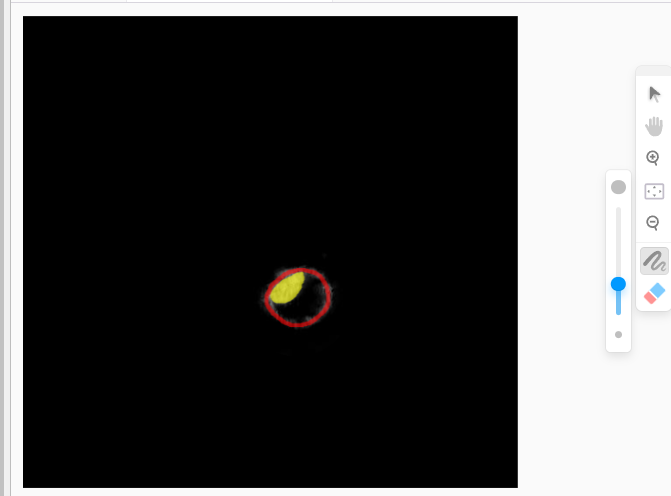
\includegraphics[scale= 0.2]{bab3/label-studio.png}
%	\caption{Proses Pembuatan Citra Mask Menggunakan \textit{Label Studio}}
%	\label{fig:label-studio}
%\end{figure}
%
%\begin{figure}[htbp]
%	\centering
%	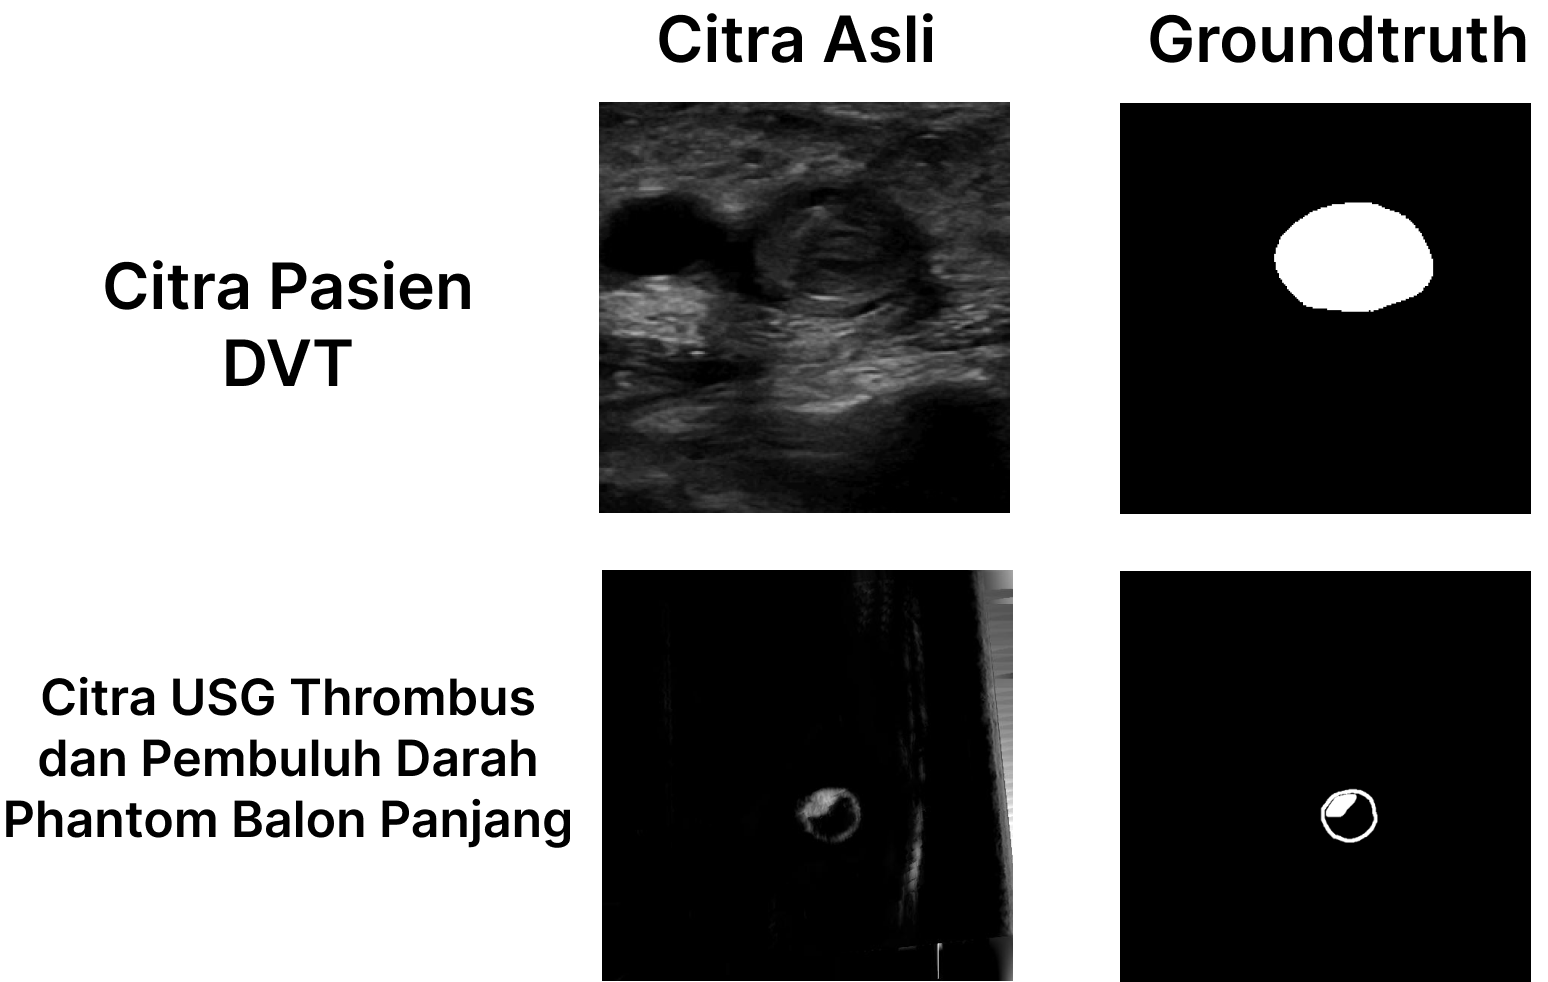
\includegraphics[scale= 0.1]{bab3/Hasil-Label.png}
%	\caption{Proses Pembuatan Citra Mask Menggunakan \textit{Label Studio}}
%	\label{fig:result-label}
%\end{figure}


Kemudian, khusus untuk citra 2D \textit{ultrasound} pembuluh darah dan \textit{thrombus} dari hasil \textit{slicing} citra 3D hasil rekonstruksi beserta citra \textit{mask}nya akan disusun kembali menjadi bentuk 3D berdasarkan urutan waktunya. Penyusunan kembali menjadi bentuk 3D ini digunakan untuk proses \textit{training} untuk membuat model segmentasi 3D. 

 
 

% \subsection{Menghapus Noise}
% Sebelum melakukan proses training data menggunakan model deep learning, citra 2D USG gumpalan darah pasien penderita DVT akan melalui proses menghapus \textit{noise}. Citra USG memiliki \textit{noise} yang tinggi. Sehingga pada penelitian ini dilakukan tahap peningkatan kualitas citra menggunakan filter \textit{gaussian}. Alasan memilih filter gaussian yang Pada penelitian ini karena berdasarkan penelitian sebelumnya, filter gaussian mampu mengurangi \textit{noise} secara detail serta membantu meningkatkan optimasi hasil segmentasi. Hasil citra 2D USG gumpalan darah yang telah melalui tahap penghapusan \textit{noise} dengan menggunakan filter \textit{gaussian}, akan melalui tahap pelabelan \textit{ground truth} area gumpalan darah.

% \subsection{Pelabelan \textit{Ground Truth} Area \textit{Thrombus}}
% Pelabelan \textit{ground truth} area citra gumpalan darah (\textit{thrombus}) digunakan sebagai citra label pada proses \textit{training} menggunakan model \textit{deep learning} U-Net. Tujuan utama pelabelan citra adalah untuk mengenali dan membedakan objek atau area yang berbeda dalam citra tersebut. Proses pelabelan pada penelitian ini menggunakan aplikasi \textit{label studio} yang bersifat \textit{open source}. Proses pelabelan area gumpalan darah vena pada citra 2D \textit{ultrasound} memberi label \textit{masking} pada area gumpalan darah. Hasil dari pelabelan tersebut menghasilkan citra \textit{mask} yang berwarna hitam putih. Warna hitam pada citra \textit{mask} menandakan bahwa bukan termasuk area gumpalan darah. Sedangkan warna putih pada citra \textit{mask} menandakan area gumpalan darah. Kemudian hasil pelabelan akan disimpan menjadi file citra baik format .PNG, .JPG, .Tiff, dan lain - lain. Adapun hasil pelabelan citra 2D gumpalan darah \textit{ultrasound} dari pasien penderita DVT dapat dilihat pada Gambar \ref{fig:labelling}. 

% \begin{figure}[H]
% 	\centering
% 	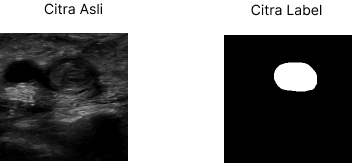
\includegraphics[scale= 0.6]{bab3/label.png}
% 	\caption{Hasil Pelabelan Citra 2D USG Gumpalan Darah Vena}
% 	\label{fig:labelling}
% \end{figure}

% digunakan sebagai dataset pelatihan (\textit{training}) dengan menggunakan model U-Net. 
%\section{Model V-Net}
%Model V-Net dapat digunakan dalam proses segmentasi guna membantu dalam identifikasi posisi gumpalan darah yang akurat. Data yang digunakan dalam proses training menggunakan model V-Net adalah hasil preprocessing citra 3D USG gumpalan darah yang telah dilakukan sebelumnya.
%\subsection{Fitur Warna}
%\lipsum[1]
%\subsection{Fitur Permukaan}
\section{Segmentasi Gumpalan Darah}
Pada tahap utama segmentasi gumpalan darah vena terdapat tiga tahapan yaitu (1) \textit{training} menggunakan model \textit{deep learning} U-Net; (2) ekstraksi fitur citra input pada \textit{encoder} U-Net; dan (3) segmentasi gumpalan darah vena pada \textit{decoder} U-Net.

\subsection{Pembagian Data Sebelum Segmentasi}
Pada proses pelatihan (\textit{training}) menggunakan 2 data citra \textit{ultrasound} yaitu citra 3D \textit{ultrasound} pembuluh darah dan \textit{thrombus} phantom balon panjang dari hasil rekosntruksi dan citra 2D \textit{thrombus} lima pasien penderita DVT. Citra 3D \textit{ultrasound} pembuluh darah dan \textit{thrombus} phantom balon panjang dari hasil rekosntruksi dapat dilakukan segementasi dengan 2 cara yaitu segmentasi 2D dan 3D. Untuk melakukan segmentasi 2D, data citra 3D \textit{ultrasound} pembuluh darah dan \textit{thrombus} phantom balon panjang dari hasil rekonstruksi akan di \textit{slice} menjadi citra 2D. Jumlah citra 3D \textit{ultrasound} yang digunakan untuk proses \textit{training} yaitu berjumlah 4 citra. Kemudian jumlah citra 2D hasil \textit{slice} citra 3D \textit{ultrasound} pembuluh darah dan \textit{thrombus} phantom balon panjang berjumlah 389 citra. Sedangkan jumlah citra 2D \textit{ultrasound} \textit{thrombus} pasien DVT berjumlah 312 citra. 

Sebelum proses pelatihan data dilakukan, ketiga citra tersebut akan dibagi menjadi dua jenis data yaitu data pelatihan (\textit{train}) dan data validasi (\textit{validation}). Data \textit{train} merupakan bagian terbesar dari dataset yang digunakan untuk melatih model. Semakin banyak data \textit{train} yang berkualitas dan bervariasi, semakin baik model segmentasi dapat mempelajari karakteristik yang lebih kompleks. Kemudian data \textit{validation} merupakan data yang digunakan untuk mengevaluasi kinerja model segemntasi selama proses pelatihan (\textit{training}). Hal tersebut bertujuan untuk memeriksa apakah model segmentasi mengalami \textit{overfitting}. Data \textit{validation} harus berbeda dari data \textit{train} tetapi masih mewakili distribusi yang sama. Adapun pembagian data citra 3D \textit{ultrasound} pembuluh darah dan \textit{thrombus} \textit{phantom} balon panjang dari hasil rekonstruksi mengacu pada Tabel \ref{tab:pembagian_data_citra_3d_rekonstruksi}.

% Please add the following required packages to your document preamble:
% \usepackage{graphicx}
\begin{table}[htbp]
	\centering
	\caption{Pembagian data citra 3D \textit{ultrasound} pembuluh darah dan \textit{thrombus} \textit{phantom} balon panjang}
	\label{tab:pembagian_data_citra_3d_rekonstruksi}
	\resizebox{\textwidth}{!}{%
		\renewcommand{\arraystretch}{2.0} % Menyesuaikan tinggi baris (1 adalah default, nilai yang lebih besar untuk lebih banyak ruang)
		\setlength{\tabcolsep}{10pt} % Menyesuaikan padding horizontal (nilai default biasanya 6pt)
		\begin{tabular}{|l|l|c|c|}
			\hline
			\multicolumn{1}{|c|}{\textbf{Pembagian}} & \multicolumn{1}{c|}{\textbf{Deskripsi}}             & \textbf{Jumlah} & \textbf{Rasio} \\ \hline
			\textbf{Data pelatihan}                  & Bagian data yang digunakan untuk melatih model      & 4               & 80\%           \\ \hline
			\textbf{Data validasi}                   & Bagian data yang digunakan untuk mengevaluasi model & 1               & 20\%           \\ \hline
		\end{tabular}%
	}
\end{table}

Kemudian, pembagian data citra 2D hasil \textit{slice} citra 3D \textit{ultrasound} pembuluh darah dan \textit{thrombus} \textit{phantom} balon panjang dari hasil rekonstruksi mengacu pada Tabel \ref{tab:pembagian_data_citra_2d_rekonstruksi}

\begin{table}[htbp]
	\centering
	\caption{Pembagian data citra 2D hasil \textit{slice} citra 3D \textit{ultrasound} pembuluh darah dan \textit{thrombus} \textit{phantom} balon panjang}
	\label{tab:pembagian_data_citra_2d_rekonstruksi}
	\resizebox{\textwidth}{!}{%
		\renewcommand{\arraystretch}{2.0} % Menyesuaikan tinggi baris (1 adalah default, nilai yang lebih besar untuk lebih banyak ruang)
		\setlength{\tabcolsep}{10pt} % Menyesuaikan padding horizontal (nilai default biasanya 6pt)
		\begin{tabular}{|l|l|c|c|}
			\hline
			\multicolumn{1}{|c|}{\textbf{Pembagian}} & \multicolumn{1}{c|}{\textbf{Deskripsi}}             & \textbf{Jumlah} & \textbf{Rasio} \\ \hline
			\textbf{Data pelatihan}                  & Bagian data yang digunakan untuk melatih model      & 310               & 80\%           \\ \hline
			\textbf{Data validasi}                   & Bagian data yang digunakan untuk mengevaluasi model & 79               & 20\%           \\ \hline
		\end{tabular}%
	}
\end{table}

Pembagian data citra 2D \textit{ultrasound} \textit{thrombus} pasien penderita DVT mengacu pada Tabel \ref{tab:pembagian_data_citra_2d_ori}

\begin{table}[htbp]
	\centering
	\caption{Pembagian data citra 2D \textit{ultrasound} \textit{thrombus} pasien penderita DVT.}
	\label{tab:pembagian_data_citra_2d_ori}
	\resizebox{\textwidth}{!}{%
		\renewcommand{\arraystretch}{2.0} % Menyesuaikan tinggi baris (1 adalah default, nilai yang lebih besar untuk lebih banyak ruang)
		\setlength{\tabcolsep}{10pt} % Menyesuaikan padding horizontal (nilai default biasanya 6pt)
		\begin{tabular}{|l|l|c|c|}
			\hline
			\multicolumn{1}{|c|}{\textbf{Pembagian}} & \multicolumn{1}{c|}{\textbf{Deskripsi}}             & \textbf{Jumlah} & \textbf{Rasio} \\ \hline
			\textbf{Data pelatihan}                  & Bagian data yang digunakan untuk melatih model      & 250               & 80\%           \\ \hline
			\textbf{Data validasi}                   & Bagian data yang digunakan untuk mengevaluasi model & 62               & 20\%           \\ \hline
		\end{tabular}%
	}
\end{table} 

%Model V-Net dapat digunakan dalam proses segmentasi guna membantu dalam identifikasi posisi gumpalan darah yang akurat. Data yang digunakan dalam proses training menggunakan model V-Net adalah hasil reduksi noise citra 3D USG gumpalan darah yang telah dilakukan sebelumnya. Output dari prediksi model V-Net adalah citra mask pada area gumpalan darah pada pembuluh darah vena. Pada arsitektur V-Net terdiri dari bagian kiri dan kanan jaringan. Penggabungan bagian kiri dan kanan pada model V-Net dalam pembuatan prediksi hasil segmentasi citra dengan cara mengeksrak fitur dari citra input dan mengubah fitur tersebut menjadi hasil prediksi yang spesifik dengan memperbesar ukuran citra. 
\subsection{Training Deep Learning Model U-Net}
Pada penelitian ini model U-Net dipilih oleh peneliti guna melakukan segmentasi area gumpalan darah (\textit{thrombus}) pada pembuluh darah vena. Proses pelatihan (\textit{training}) dalam kasus segmentasi citra menggunakan model \textit{deep learning} seperti U-Net adalah untuk mengajarkan model tersebut bagaimana mengidentifikasi dan membedakan objek target dimana dalam kasus peneliti pada gumpalan darah (\textit{thrombus}) pada pembuluh darah vena. Dalam proses segmentasi, penelitian ini menggunakan bahasa pemrograman \textit{Python} versi 3 yang dijalankan melalui \textit{platform Google Colab}. Adapun spesifikasi \textit{platform Google Colab} dapat dilihat pada Tabel \ref{tab:spesifikasi_platform_google_colab}.


\begin{table}[htbp]
	\centering
	\caption{Spesifikasi platform Google Colab}
	\label{tab:spesifikasi_platform_google_colab}
	\resizebox{\textwidth}{!}{%
		\renewcommand{\arraystretch}{2.0} % Menyesuaikan tinggi baris (1 adalah default, nilai yang lebih besar untuk lebih banyak ruang)
		\setlength{\tabcolsep}{10pt}
		\begin{tabular}{|l|l|}
			\hline
			\textbf{CPU}         & AMD EPYC 7B12 (2,24 GHz) \\ \hline
			\textbf{GPU}         & Tesla T4                 \\  \hline
			\textbf{RAM}         & 12,7 GB                  \\  \hline
			\textbf{Penyimpanan} & 166,8 GB                 \\ \hline
		\end{tabular}%
	}
\end{table}

Dalam proses \textit{training} juga ada beberapa konfigurasi yang didefinisikan oleh peneliti. Adapun konfigurasi pelatihan yang didefinisikan oleh peneliti mengacu pada Tabel \ref{tab:konfigurasi_hiperparameter_model}.


\begin{table}[htbp]
	\centering
	\caption{Konfigurasi Hiperparameter Model}
	\label{tab:konfigurasi_hiperparameter_model}
	\resizebox{\textwidth}{!}{%
		\renewcommand{\arraystretch}{2.0} % Menyesuaikan tinggi baris (1 adalah default, nilai yang lebih besar untuk lebih banyak ruang)
		\setlength{\tabcolsep}{10pt}
		\begin{tabular}{|l|l|}
			\hline
			\textbf{Batch Size}                           & 8                   \\ \hline
			\textbf{Epoch}                                & 100                 \\ \hline
			\textbf{Tingkat Pembelajaran (Learning Rate)} & 0,0001              \\ \hline
			\textbf{Pengoptimalan (Optimizer)}            & Adam                \\ \hline
			\textbf{Loss}                                 & Binary Crossentropy \\ \hline
			\textbf{Aktivasi Layer}                       & Softmax             \\ \hline
			\textbf{Kelas}                                & 2                   \\ \hline
		\end{tabular}%
	}
\end{table}

Hasil segmentasi akan dievaluasi menggunakan 5 \textit{metric} evaluasi sebagai berikut (1)\textit{accuracy}; (2)\textit{loss}; (3)\textit{Intersection over Union} (IoU); (4)\textit{dice coefficient}; dan (5) \textit{hausdorff distance}. \textit{Metric} evaluasi \textit{accuracy} berfungsi untuk menghitung nilai prediksi yang tepat terhadap data yang memiliki area gumpalan darah \textit{thrombus} pada pembuluh darah vena yang diperoleh melalui model segmentasi U-Net pada saat proses \textit{training}. Nilai persentase \textit{accuracy} yang tinggi menunjukkan bahwa model yang dihasilkan lebih akurat dalam melakukan segmentasi citra \textit{ultrasound} \textit{thrombus}.

Metrik evaluasi \textit{loss} berfungsi untuk menghitung nilai kesalahan model segmentasi dalam memprediksi data citra yang memiliki area \textit{thrombus} pada saat proses \textit{training}. Nilai \textit{loss} yang rendah menunjukkan nilai kesalahan yang kecil antara citra prediksi dan \textit{groundtruth} dari citra \textit{ultrasound thrombus}. Metrik evaluasi \textit{Intersection over Union (IoU)} berfungsi untuk mengukur kemiripan antara dua objek dalam citra. Dalam kasus pada penelitian ini, pengukuran kemiripan antara \textit{ground truth} dari citra \textit{ultrasound} \textit{thrombus} dan citra prediksi \textit{thrombus} yang dihasilkan melalui proses segmentasi. Nilai IoU memiliki rentang 0 hingga 1. Apabila nilai IoU mendekati 0, maka citra hasil prediksi segmentasi tidak mirip dengan bentuk dari \textit{groundtruth}. Sedangkan jika nilai IoU mendekati 1, maka citra hasil prediksi segmentasi mirip dengan bentuk dari \textit{groundtruth}. \textit{Metric} evaluasi \textit{dice coefficient} memiliki fungsi yang sama dengan \textit{metric} evaluasi IoU yaitu mengukur kemiripan antara dua objek dalam citra. \textit{Dice coefficient} memiliki rentang 0 hingga 1. \textit{Dice coefficient} dipilih peneliti karena sensitivitasnya terhadap perubahan kecil dalam area segmentasi. Nilai \textit{hausdroff distance} diperoleh melalui perhitungan nilai 2 titik terjauh pada 2 citra. Di dalam penelitian ini, \textit{haudorff distance} diterapkan pada pengukuran antara \textit{groundtruth} dan hasil prediksi segmentasi. Nilai \textit{hausdorff distance} akan bernilai 0 jika himpunan kedua titik (\textit{groundtruth} dan hasil prediksi segmentasi) memiliki kesamaan. Sedangkan apabila nilai \textit{hausdorff distance} memiliki nilai yang tinggi, maka himpunan kedua titik (\textit{groundtruth} dan hasil prediksi segmentasi) tersebut memiliki jarak yang berjauhan. Hasil uji performa kedua model tersebut akan dijelaskan pada Bab 4.
%Pembagian data pada proses \textit{training}, Seluruh data dibagi sebesar 80\% yang digunakan untuk data \textit{train} sedangkan sebesar 20\% akan digunakan sebagai data \textit{validation}. Data \textit{train} berjumlah 254 citra serta data \textit{validation} berjumlah 63 citra.

%Matriks evaluasi pada penelitian ini menggunakan \textit{Intersection over Union} (IoU Score). Metode IoU score memiliki beberapa karakteristik yang sesuai dengan kebutuhan evaluasi model segmentasi dengan karakteristik sebagai berikut:

%\begin{enumerate}
%    \item Intuitif: Nilai IoU adalah persentase \textit{overlap} antara area objek yang sebenarnya dan area yang dihasilkan oleh model segmentasi. Ini mudah dipahami dan mudah digunakan untuk mengevaluasi kinerja model segmentasi.
%    \item Fleksibel : Nilai IoU dapat digunakan untuk berbagai jenis bentuk dari citra itu sendiri. Seperti objek persegi, lingkaran, atau poligon
%    \item \textit{Robust} : Nilai IoU digunakan untuk menghitung luas overlap antara area objek sebenarnya dan area yang dihasilkan oleh model segmentasi. 
%    \item Konsisten : Nilai IoU digunakan untuk memberikan konsistensi dalam mengevaluasi kinerja model segmentasi
%    \item Memperhitungkan false positive dan false negative
%\end{enumerate}

%Jumlah nilai IoU yang lebih tinggi menunjukkan bahwa sistem segmentasi bekerja dengan baik dalam menemukan objek dalam citra. Proses pengukuran IoU terdiri dari menghitung luas overlap antara area objek yang sebenarnya dan area yang dihasilkan oleh sistem segmentasi, lalu dibandingkan dengan luas total area objek yang sebenarnya dan area yang dihasilkan oleh sistem segmentasi.

\subsection{Ekstraksi Fitur Citra Input pada Encoder U-Net}
Pada penelitian ini dilakukan segmentasi 2D dan 3D menggunakan model U-Net. Pada arsitektur U-Net terdapat bagian \textit{encoder} dan \textit{decoder}. Model U-Net menggabungkan bagian \textit{encoder} dan \textit{decoder} untuk membuat prediksi segmen citra dengan mengekstrak fitur tersebut menjadi prediksi segmen yang lebih spesifik yang memperbesar ukuran citra. Pada segmentasi 2D, input citra 2D ultrasound akan melalui bagian \textit{encoder} model U-Net untuk proses ekstraksi fitur - fitur pada citra tersebut. Berikut ini ilustrasi citra input pada model U-Net2D dengan hasil output citra \textit{mask} area gumpalan darah dapat dilihat pada Gambar \ref{fig:modelU-Net2D}.

\begin{figure}[htbp]
	\centering
	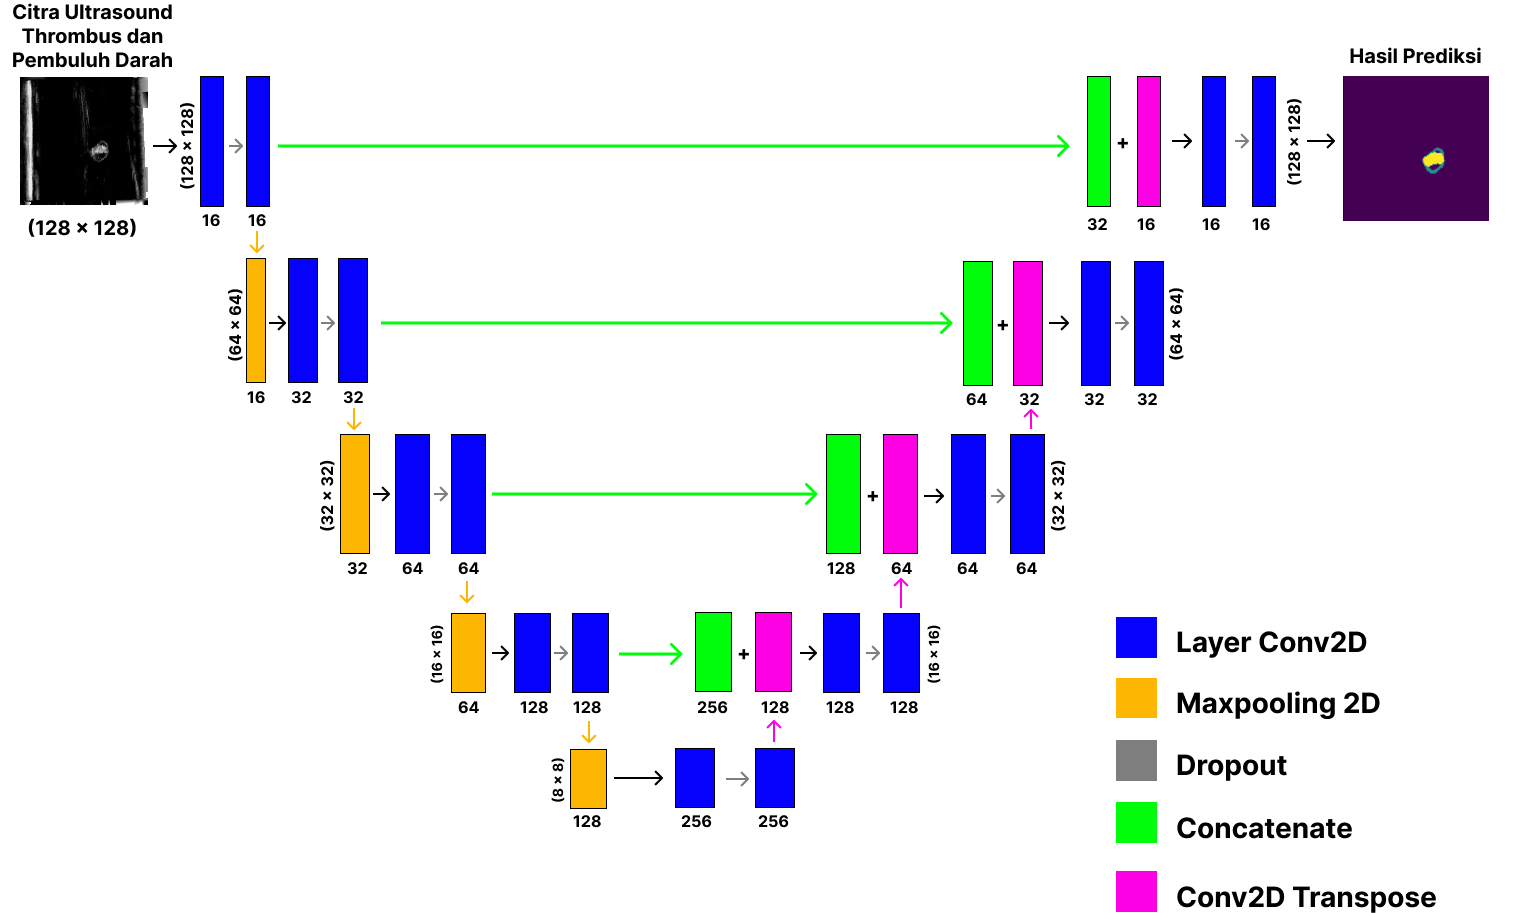
\includegraphics[scale= 0.2]{bab3/unet_2d.png}
	\caption{Arsitektur U-Net 2D}
	\label{fig:modelU-Net2D}
\end{figure}

Masing - masing layer pada \textit{encoder} model U-Net akan mengimplementasikan filter \textit{convolutional} terhadap citra input. Kemudian citra input akan di \textit{pooling} sehingga ukuran dimensinya menjadi berkurang serta mengekstrak fitur yang lebih abstrak. Proses ini berlangsung hingga tahap akhir bagian \textit{encoder}. Fitur yang dihasilkan oleh \textit{encoder} akan digunakan sebagai input pada bagian \textit{decoder}. Pada bagian \textit{encoder} U-Net akan dilakukan uji coba modifikasi menggunakan model \textit{pre-trained} VGG16 untuk meningkatkan performa ekstraksi fitur citra input. Uji coba performa model \textit{pre-trained} VGG16 dan U-Net akan dibandingkan dengan model U-Net standar.

Kemudian pada segmentasi 3D, input citra 3D \textit{ultrasound} akan melalui bagian \textit{encoder} model U-Net3D untuk proses eksraksi fitur - fitur pada citra tersebut. Adapun yang membedakan dari model U-Net2D dan U-Net3D terletak pada inputan citranya, layer konvolusi, layer \textit{maxpooling}, serta layer \textit{transpose}. Pada model U-Net3D, inputan citra layer konvolusi, layer \textit{maxpooling}, serta layer \textit{transpose} semua dalam bentuk 3 dimensi. Berikut ini ilustrasi citra input pada model U-Net3D dengan hasil output citra \textit{mask} area gumpalan darah dapat dilihat pada Gambar \ref{fig:model_U-Net3D}.  

\begin{figure}[htbp]
	\centering
	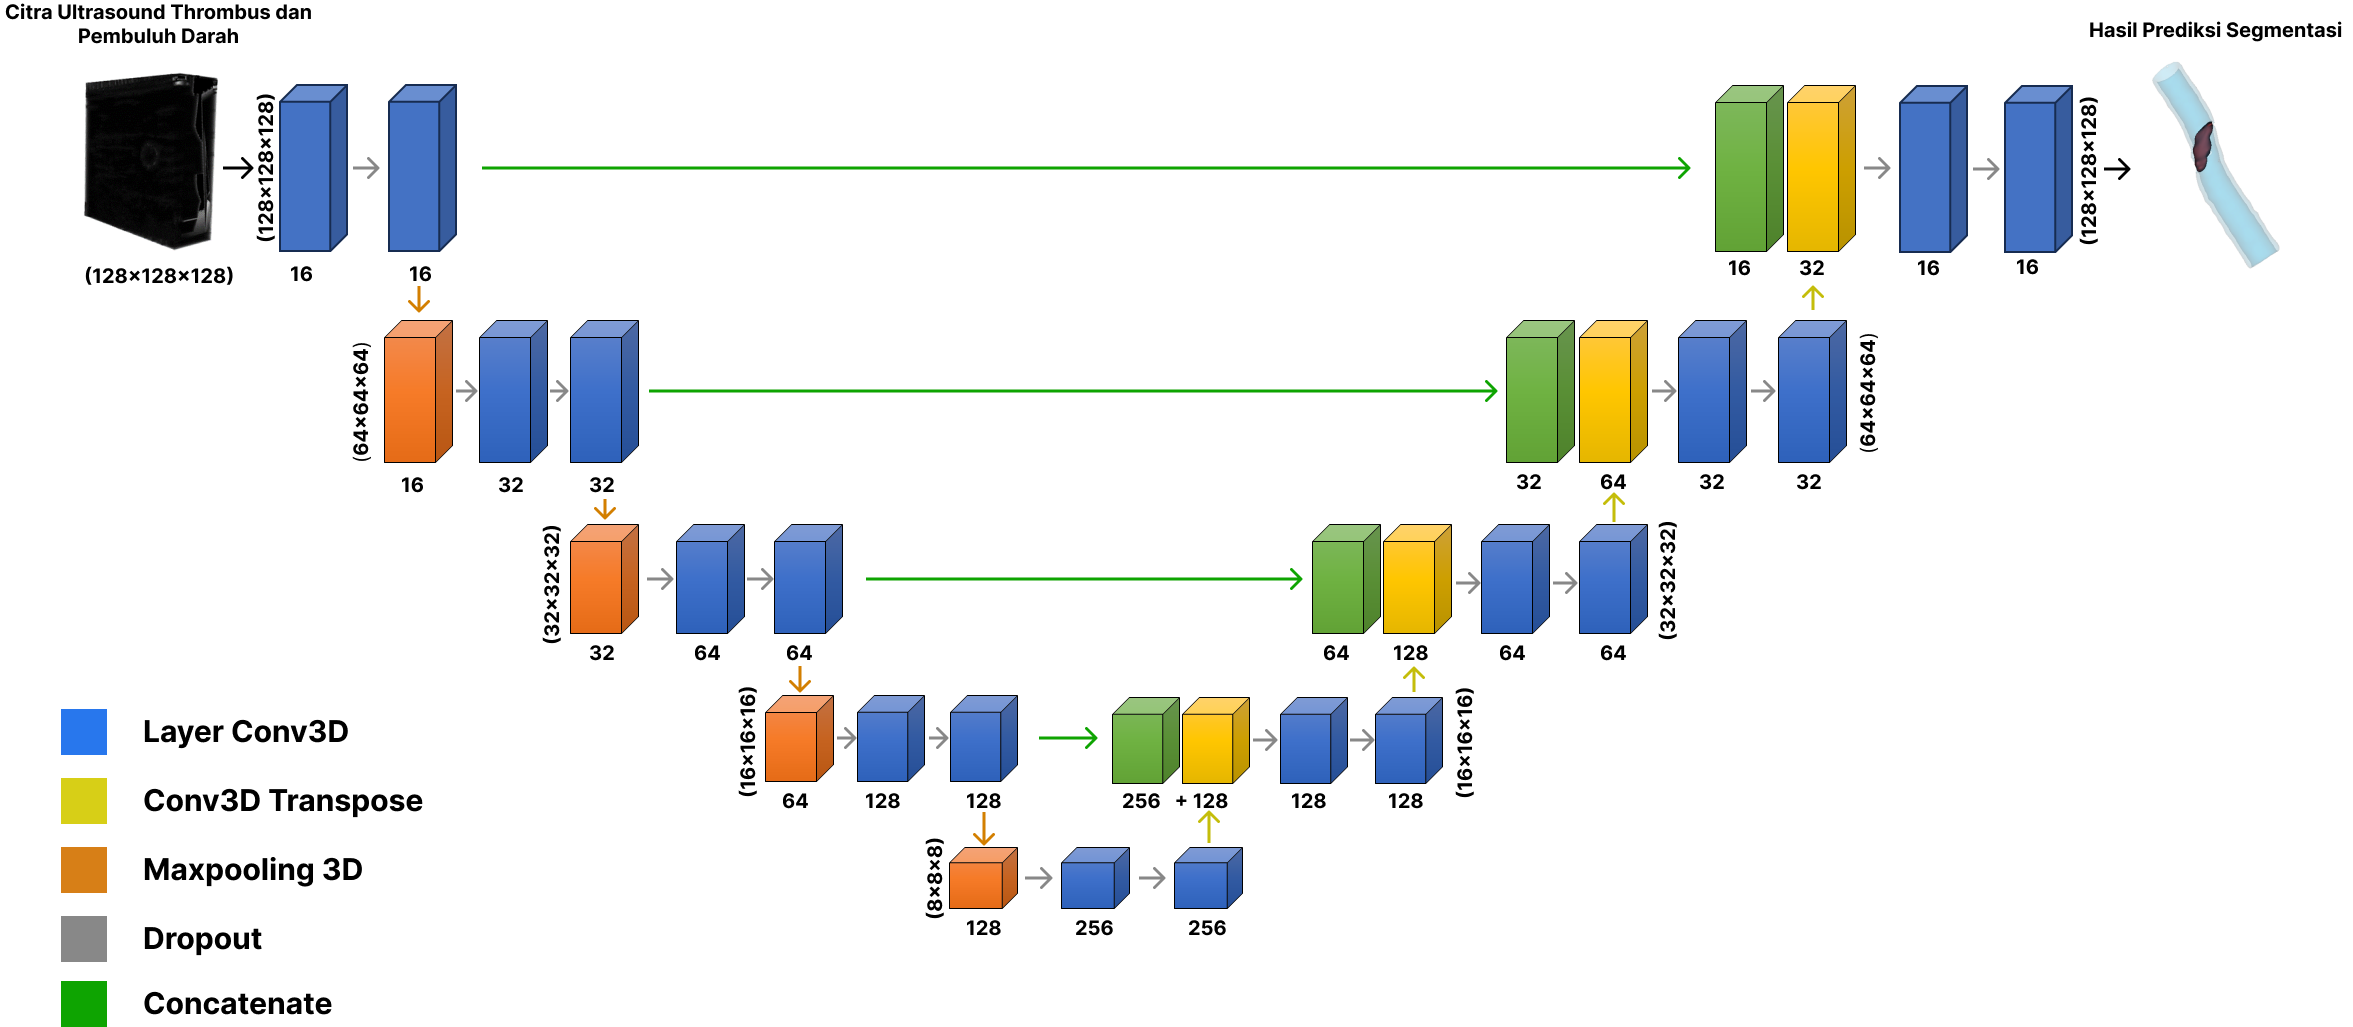
\includegraphics[scale= 0.2]{bab3/Unet 3d.png}
	\caption{Arsitektur U-Net 3D}
	\label{fig:model_U-Net3D}
\end{figure}


Hasil performa segmentasi dari kedua model tersebut akan dievaluasi menggunakan 5 metrik evaluasi yaitu \textit{accuracy}, \textit{loss}, \textit{Intersection over Union} IoU, \textit{dice coefficient}, \textit{hausdorff distance}.

\subsection{Segmentasi Gumpalan Darah Vena pada \textit{Decoder} U-Net}
Kemudian output dari hasil ekstraksi pada bagian \textit{encoder} akan menjadi input pada bagian \textit{decoder} model U-Net. Pada bagian \textit{decoder} berfungsi untuk mengubah fitur dari bagian \textit{encoder} menjadi prediksi segmen citra. Bagian ini menggunakan layer \textit{transposed} untuk meningkatkan ukuran citra yang dihasilkan pada layer sebelumnya. Setiap layer pada bagian \textit{decoder} akan menggabungkan fitur dari layer sebelumnya guna membuat prediksi segmen area gumpalan darah (\textit{thrombus}). Proses ini dilakukan hingga layer terakhir bagian \textit{decoder}.

%\section{Visualisasi Gumpalan Vena 3D}
\section{Skenario Pada Penelitian}

Dalam rangka membuat model yang lebih efisien dan akurat untuk segmentasi gumpalan darah \textit(thrombus) vena pada citra \textit{ultrasound}, penelitian ini telah dirancang dengan lima skenario penelitian yang berbeda. Setiap skenario dikembangkan untuk mengeksplorasi dan menilai penggunaan model U-Net standar dan model \textit{pre-trained} VGG16 dan U-Net dalam konteks segmentasi 2D dan 3D. Skenario pada penelitian ini dapat dilihat pada Gambar \ref{fig:skenario_penelitian}.


\begin{figure}[htbp]
	\centering
	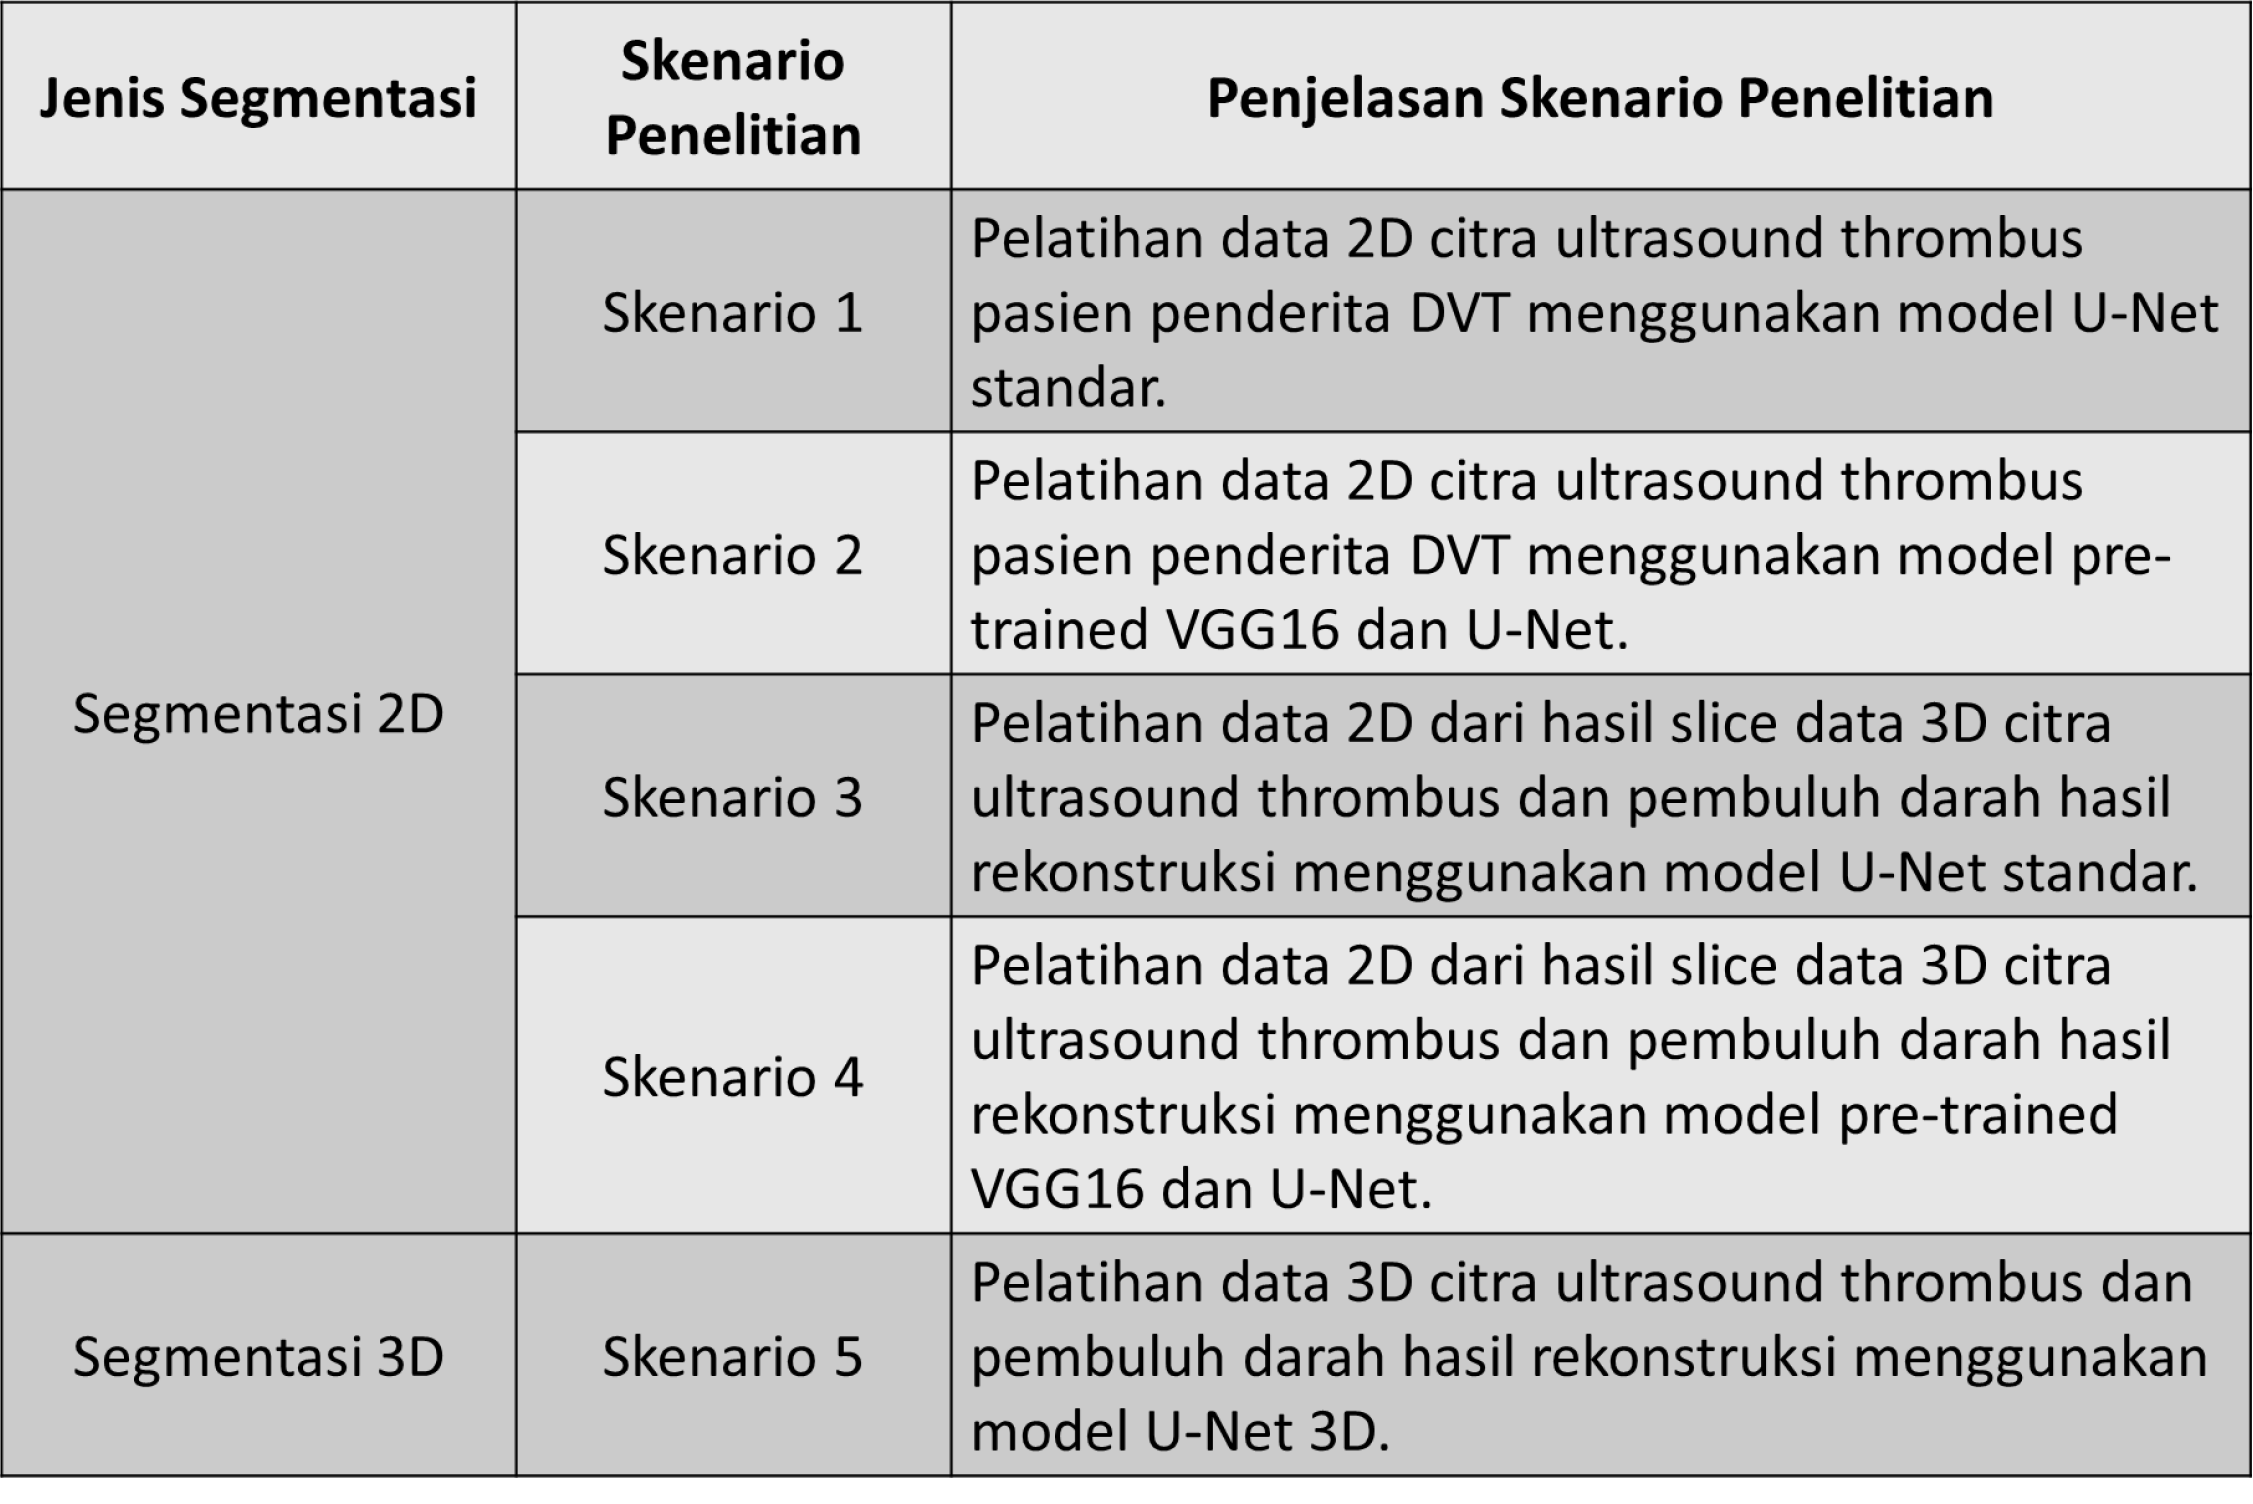
\includegraphics[scale= 0.2]{bab3/skenario_penelitian.png}
	\caption{Skenario Pada Penelitian}
	\label{fig:skenario_penelitian}
\end{figure}

Untuk data citra \textit{ultrasound} di setiap skenario pada segmentasi 2D akan dilakukan reduksi \textit{noise} dengan menggunakan 5 filter \textit{denoising} yaitu (1) filter \textit{gaussian}; (2) filter \textit{median}; (3) filter \textit{mean}; (4) filter \textit{bilateral}; dan (5) filter \textit{non local means}. Hasil pelatihan pada setiap skenario akan di evaluasi menggunakan 5 metrik evaluasi yaitu \textit{accuarcy}, \textit{loss}, \textit{IoU}, \textit{dice coefficient}, dan \textit{hausdorff distance}.


%\lipsum[4]
%\section{Segmentasi Gumpalan Darah}
%\lipsum[2]






